\PassOptionsToPackage{unicode=true}{hyperref} % options for packages loaded elsewhere
\PassOptionsToPackage{hyphens}{url}
%
\documentclass[11pt,]{article}
\usepackage[]{mathpazo}
\usepackage{amssymb,amsmath}
\usepackage{ifxetex,ifluatex}
\usepackage{fixltx2e} % provides \textsubscript
\ifnum 0\ifxetex 1\fi\ifluatex 1\fi=0 % if pdftex
  \usepackage[T1]{fontenc}
  \usepackage[utf8]{inputenc}
  \usepackage{textcomp} % provides euro and other symbols
\else % if luatex or xelatex
  \usepackage{unicode-math}
  \defaultfontfeatures{Ligatures=TeX,Scale=MatchLowercase}
\fi
% use upquote if available, for straight quotes in verbatim environments
\IfFileExists{upquote.sty}{\usepackage{upquote}}{}
% use microtype if available
\IfFileExists{microtype.sty}{%
\usepackage[]{microtype}
\UseMicrotypeSet[protrusion]{basicmath} % disable protrusion for tt fonts
}{}
\IfFileExists{parskip.sty}{%
\usepackage{parskip}
}{% else
\setlength{\parindent}{0pt}
\setlength{\parskip}{6pt plus 2pt minus 1pt}
}
\usepackage{hyperref}
\hypersetup{
            pdftitle={Patterns of agricultural intensification drive bumble bee occurrence in the North American Midwest},
            pdfauthor={Jeremy Hemberger; Michael Crossley; Claudio Gratton},
            pdfkeywords={Agricultural intensification, Bumble bees, bee decline, agroecosystems},
            pdfborder={0 0 0},
            breaklinks=true}
\urlstyle{same}  % don't use monospace font for urls
\usepackage[margin = 1in]{geometry}
\usepackage{graphicx,grffile}
\makeatletter
\def\maxwidth{\ifdim\Gin@nat@width>\linewidth\linewidth\else\Gin@nat@width\fi}
\def\maxheight{\ifdim\Gin@nat@height>\textheight\textheight\else\Gin@nat@height\fi}
\makeatother
% Scale images if necessary, so that they will not overflow the page
% margins by default, and it is still possible to overwrite the defaults
% using explicit options in \includegraphics[width, height, ...]{}
\setkeys{Gin}{width=\maxwidth,height=\maxheight,keepaspectratio}
\setlength{\emergencystretch}{3em}  % prevent overfull lines
\providecommand{\tightlist}{%
  \setlength{\itemsep}{0pt}\setlength{\parskip}{0pt}}
\setcounter{secnumdepth}{0}
% Redefines (sub)paragraphs to behave more like sections
\ifx\paragraph\undefined\else
\let\oldparagraph\paragraph
\renewcommand{\paragraph}[1]{\oldparagraph{#1}\mbox{}}
\fi
\ifx\subparagraph\undefined\else
\let\oldsubparagraph\subparagraph
\renewcommand{\subparagraph}[1]{\oldsubparagraph{#1}\mbox{}}
\fi

% set default figure placement to htbp
\makeatletter
\def\fps@figure{htbp}
\makeatother

\usepackage{setspace}\doublespacing
\usepackage[left]{lineno}
\linenumbers
\usepackage{dcolumn}
\usepackage{caption}
\usepackage{float}
\usepackage{afterpage}
\usepackage{siunitx}
\usepackage{amsmath}

\title{\textbf{Patterns of agricultural intensification drive bumble bee
occurrence in the North American Midwest}}
\author{Jeremy Hemberger \and Michael Crossley \and Claudio Gratton}
\date{September 23, 2020}

\begin{document}
\maketitle
\begin{abstract}
Recently documented insect declines suggest that agricultural expansion
and productivity-focused intensification are a putative driver for the
observed declines. However, this hypothesis has yet to be formally
tested due to a lack of historical data on agricultural land-use change
and insect taxa. Using large, spatiotemporal sets of bumble bee and
agricultural records, we show that agricultural intensification,
specifically an increase cropland extent and insecticides, as well as a
decrease in crop richness and perennial habitat, are associated with a
decrease in the occurrence of bumble bee species in the agriculturally
intensive Midwest. Yet, we found positive associations between bumble
bees and crop richness and pasture, even in areas where agriculture is
spatially extensive. Our findings suggest that insect conservation and
agricultural production may be compatible, with increasing in on-farm
and landscape-level crop diversity, pasture, and reduction in
insecticides predicted to have positive effects on bumble bees.
\end{abstract}

\captionsetup[table]{labelformat=empty}

\hypertarget{introduction}{%
\section{Introduction}\label{introduction}}

Agriculture is a primary way in which humans alter terrestrial
landscapes and is cited as a principle cause of biodiversity declines
worldwide (Foley et al. 2005, 2011, Klein et al. 2007, Tilman et al.
2011, Tscharntke et al. 2012). In particular, the intensification of
agriculture, that is, the widespread planting of crop monocultures,
managed for high productivity promoted by fertilizers and pesticides,
and high disturbance agronomic practices such as tillage, has been
associated with the extensive loss of a number of ecosystem service
providing taxa (Benton et al. 2002, Robinson and Sutherland 2002, Meehan
et al. 2010). There is circumstantial evidence that agricultural
practices are an important driver of the recently documented,
large-scale decline of insects (Hallmann et al. 2017, Seibold et al.
2019). Pollinating insects, specifically bees, may be particularly
impacted, sounding alarms across the world to consider the consequences
for natural and agricultural systems (Steffan-Dewenter et al. 2005,
Tylianakis 2013).

Bumble bees (Apidae: \emph{Bombus}) are a well-studied bee taxon that
includes many species documented to be declining across Europe and
North/South America (Biesmeijer 2006, Colla and Packer 2008, Grixti et
al. 2009, Cameron et al. 2011, Bartomeus et al. 2013, Morales et al.
2013, Wood et al. 2019). Of several putative drivers of bumble bee
decline including climate change (Kerr et al. 2015, Soroye et al. 2020)
and pathogens (Cameron et al. 2011, Szabo et al. 2012). many studies
point to agricultural intensification as another key driver of bumble
bee population decline (Grixti et al. 2009, Goulson et al. 2015).
Intensification includes both attributes within a farming system (i.e.,
pesticide use, number and types of crops used), and the effects on
agricultural landscapes (i.e., amount of land in cultivation compared to
natural habitats not used for agriculture). Despite the hypothesized
threat of agricultural intensification to bumble bees, no studies have
specifically tested the hypothesis that long-term patterns of changes in
agriculture are associated with changes in bumble bee occurrence. In
general, this is due to a paucity of long-term data of both bumble bee
occurrence and historical agricultural patterns at sufficiently large
spatial scales.

While contemporary studies examining bumble bee responses to agriculture
provide some insights, historical data from archives such as museum
records, are important tools to explore patterns of bumble bee change
over the course of decades, and offer insights of drivers at temporal
and spatial scales that elude detailed, small-scale experimental
approaches (Meehan et al. 2011, Rosenheim and Gratton 2017). The
continued addition of records to repositories such as the Global
Biodiversity Information Facility (GBIF) combined with modern, extensive
surveys of bumble bee fauna (e.g., Bumble Bee Watch, iNaturalist) offer
widespread, species-specific spatial distribution patterns. Moreover,
analyses of records from such repositories have benefited from
analytical approaches that account for known biases in archival data
(Pearce and Boyce 2006, Bartomeus et al. 2013, 2019).

To test the hypothesis that long-term bumble bee occurrence trends are
associated with patterns of agricultural intensification, we utilized an
extensive data set of historical bumble bee museum records and modern
citizen-science surveys for the North Central USA and combined this with
a newly available digital dataset of agronomic metrics compiled from
United States Census of Agriculture over the period 1870-2018 (Crossley
et al.~\emph{in review}).

We predicted that increasing agricultural intensification, as measured
by the amount cropland and cropland treated with insecticides, would be
negatively associated with bumble bee occurrence (Goulson et al. 2008,
2015, Williams and Osborne 2009, Samuelson et al. 2018). In contrast, we
expected that features of agricultural landscapes that increase
diversity, such as higher richness of crops grown, and low intensity
agronomic practices, such as the presence of perennial landscape
features such as pastures, would be positively associated with bumble
bee occurrence (Sirami et al. 2019).

\hypertarget{results}{%
\section{Results}\label{results}}

\hypertarget{agricultural-extent-remains-similar-while-crop-richness-has-declined}{%
\subsection{Agricultural extent remains similar while crop richness has
declined}\label{agricultural-extent-remains-similar-while-crop-richness-has-declined}}

From the onset of available land-use records in the 1870s, agricultural
landcover increased rapidly and began to plateau by the early 1900s. The
areal extent of cropland peaked in the study region in 1950 (45\% ±
0.9\% of county area, mean ± standard error). Since then, it has
decreased \textasciitilde{}11\% to an average of \textbf{34\% ± 0.9\%}
in 2017 (Fig. 1A,B). There are within-region differences in agricultural
cover with northern areas of the study region remaining relatively low
in agricultural cover, while the highest intensity of agricultural cover
occurs in the ``corn belt'' that stretches through southern Minnesota,
Iowa, southern Wisconsin, central and northern Illinois, and northern
Indiana. Of the 18 crops for which we compiled data, an average of 12 ±
1 were grown per county from 1880 -- 1950. Since 1950, this number has
declined \textasciitilde{}50\%, with counties today growing on average 6
± 1 crops (Fig. 1 C,D).

The additional agricultural intensification variables that we utilized,
available for the last 3 decades, showed diverging patterns, with
proportion of pasture declining 90\% from 1982 to present from an
average of 3\% of county area in 1982 to 0.3\% in 2012, while the
proportion of total county area treated with insecticides increased 54\%
from an average of 11\% of county area in 1982 to 17\% in 2012.
\emph{(Fig. S6)}. These changes occurred over similar spatial extents,
primarily concentrated in the corn-belt counties throughout the middle
of the study region.

\hypertarget{bumble-bee-species-richness-has-declined}{%
\subsection{Bumble bee species richness has
declined}\label{bumble-bee-species-richness-has-declined}}

Rarefied species richness estimates for the study region declined
significantly over the last 130 years; 20\% over the study period from
approximately 15 to 12 species from 1824-1925 to present, respectively
(Fig. 2, Linear model: t\textsubscript{1,13} = 6.084, p = 0.0283;
Permutation test: p = 0.03). A sharp drop in estimated species richness
occurred between in the 1950s, followed by a slight rebound in the next
50 years.

\hypertarget{patterns-of-bumble-bee-occurrence-are-related-to-agricultural-intensity}{%
\section{Patterns of bumble bee occurrence are related to agricultural
intensity}\label{patterns-of-bumble-bee-occurrence-are-related-to-agricultural-intensity}}

We found strong, interacting relationships between the predicted
probability of occurrence, measures of agricultural intensity, and time,
indicating fluctuating species responses based on both the agricultural
conditions in the county and the time period. Predicted responses
revealed that the probability of species occurrence increased in
accordance with crop richness (with the exception of \emph{B.
griseocollis}) (Fig. 4, 5, Table S1). Moreover, most species, namely
\emph{B. affinis}, \emph{B. bimaculatus}, \emph{B. impatiens}, revealed
high occurrence probabilities in counties under extensive cultivation
(proportion cropland \textgreater{} 0.5), provided the number of crops
grown was high (\textgreater{} 11 crops per county).

Other species, such \emph{B. pensylvanicus}, revealed increasing
sensitivity to intensive agriculture over time. For example, probability
of occurrence in areas of historically intensive agriculture (proportion
of cropland = 0.9, number of crops \textless{} 11) has declined well
over 50\% from 1900 to present. For \emph{B. pensylvanicus}, the number
of crops had little impact in the patterns of predicted occurrence;
model predictions revealed a decrease in predicted occurrence across the
range of crop richness in our data. Similarly, \emph{B. impatiens}
revealed a strong temporal interaction between proportion cropland,
number of crops, and time, with the predicted occurrence in
agriculturally extensive areas with few crops decreasing only after the
middle of the 20th century, coincident with the rise of soybean
cultivation and decline in crop richness, generally (Fig. S4)

Our models also revealed clear spatial patterns for the expected change
in predicted species occurrence given county-level statistics of
agricultural intensification (Fig. 5A, D). When the temporal trend in
predicted occurrence is examined for each species/county, two distinct
patterns in the likelihood of occurrence emerge for species of
conservation concern, and common species, respectively (Fig. 5B, C, E,
F), with the occurrence of species of conservation concern becoming less
likely, while the other focal species become increasingly common.

For more recent years (1982-2018) when additional types of agricultural
data were available, we found that the extent of pasture and insecticide
use also impacted the predicted probability of occurrence. Again, there
were significant interactions among the agricultural metrics and time
(see Figs. S5-S10, Table S2) As with previous models, predicted
occurrence increased with increasing crop diversity, except for \emph{B.
griseocollis} (Fig. S8) and \emph{B. pensylvanicus} (Fig. S5).
Additionally, the predicted probability of occurrence increased for all
species except \emph{B. pensylvanicus} in counties with increasing
proportion pasture and decreasing coverage with insecticides, although
the predicted impact of pesticides on occurrence was notably weaker than
crop richness or proportion pasture. This pattern was particularly
apparent for, \emph{B. terricola}, whose occurrence was only predicted
in counties with high crop richness, high proportion of pasture, and low
proportion of land treated with insecticides (Fig. S7).

\hypertarget{discussion}{%
\section{Discussion}\label{discussion}}

Using bumble bee observations recorded over 130 years across 6
agriculturally important US states and a novel dataset on the historical
patterns of agricultural land use and practices, we explored the
hypothesis that agricultural intensification is associated with bumble
bee occurrence. In doing so, we take special care to account for biases
associated with historical collections and employed a variety of
techniques including subsampling and sensitivity analyses to determine
whether our chosen methods skewed results (Bartomeus et al. 2019).
Irrespective of the approaches used, we consistently identified clear
statistical associations between bumble bee species occurrence and
metrics of agricultural intensity. After accounting for temporal trends
in bumble bee occurrence, it appears that increases in agricultural
intensity in the landscape favor a select few bumble bee species at the
expense of others.

Contrary to expectations, our results suggest that the extent of
agricultural land is not the sole predictor of the fate of bumble bee
species, as the manner in which agriculture is practiced also affected
occurrence patterns. For example, our model revealed that several bumble
bee species had a high predicted probability of occurrence within
agriculturally extensive landscapes in the early 1900's. However, a
rapid decrease in crop richness from the 1930's onward was associated
with a decrease in the predicted occurrence of several bumble bees. Of
the crops included in our analyses, a large decrease occurred in cover
and hay crops, which include bumble bee food plants in the family
Fabaceae, as well as other bumble bee attractive crops including
buckwheat and pulses. Together, these changes suggest that the post-war
era intensification of agriculture, with its loss of crop diversity,
bumble bee attractive crops, pasture and increasing pesticide use
(Meehan et al. 2011, Fernandez-Cornejo et al. 2014, Meehan and Gratton
2015), rather than the areal expansion of agriculture, has been a major
driver in the shift of bumble bee communities. Indeed, these patterns
parallel the decline of insect pollinators ({\textbf{???}}, Ollerton et
al. 2014) and biodiversity (Robinson and Sutherland 2002) in the UK,
bumble bee declines in Illinois (Grixti et al. 2009), as well as
wildlife declines within the same geographic range of our study (Lark et
al. 2020). Moreover, the predicted occurrence of the majority of bumble
bee species examined was generally greater in areas of high crop
richness across the temporal span of our data, as well as perennial
cropping areas such as pasture for more recent records.

Agricultural intensification is also correlated with a decrease in the
amount of other natural habitats that support diverse floral habitat
such as grasslands (Smith 1998, Brown and Schulte 2011) and bumble bee
forage plants (Carvell et al. 2006, Scheper et al. 2014), as well as
increases insecticide use (Meehan et al. 2011, Meehan and Gratton 2015).
A shift from the diverse cropping systems of the early to mid 1900's to
largely monocultural systems in recent years has also altered the
temporal continuity of available floral resources Schellhorn et al.
(2015); Timberlake et al. (2019){]} and total pollen availability, which
has been shown to negatively impact bumble bee health (Vaudo et al.
2015, Cameron and Sadd 2020), colony growth and development (Williams et
al. 2012, Hass et al. 2018), and may be of particular concern for
species with more limited diet breadths (Kleijn and Raemakers 2008, Wood
et al. 2019). Future studies could be designed to explore, for example,
contemporary relationships between bumble bee abundance and gradients of
agricultural intensity such as crop diversity and areal amount of
agriculture to reveal a more mechanistic understanding of how select
agricultural factors are impacting bumble bee populations. Lastly,
population changes in other pollinating taxa, especially wild bees, may
also be related to the increases in agricultural intensity described
here. Compiling occurrence records for those species with sufficient
spatiotemporal data coverage would allow a more thorough assessment of
the impacts of agricultural intensification on pollinators writ large.

\emph{Paragraph here about balance of winners/losers, similar to
previous drafts?}

The patterns revealed in this analysis suggest opportunities for bumble
bee conservation within agricultural landscapes. Even landscapes with a
high areal extent of agriculture may still support both common and
declining bumble bee species provided there is a high diversity of
crops, perennial features such as pasture, and limited insecticide use.
Sirami et al. (2019) found a similar pattern for farmland biodiversity:
increasing the diversity of crops and decreasing field size had a large,
positive effect on multi-trophic indices of biodiversity. Our results
provide additional evidence that agricultural landscape heterogeneity is
key to supporting farmland biodiversity (Benton et al. 2003, Fahrig et
al. 2011). Such changes may also benefit growers struggling to profit
from the corn and soybean dominated markets of the last decade
({\textbf{???}}) by providing access to alternative commodity markets.
It is important to note, however, that the ideal agricultural conditions
for the occurrence of most bumble bee species we examined, particularly
with regard to the number of crops grown, are no longer present in
Midwestern agricultural landscapes. As of 2017, almost all counties grow
fewer than 10 crops, and most highly agricultural counties are dominated
by even a smaller subset.

Changes in agricultural intensity are unlikely to be the sole direct
cause of bumble bee declines, but are likely associated with other
impactful agricultural practices (such as pathogen spillover from
greenhouse operations, Szabo et al. 2012) or anthropogenic processes
(e.g., climate change Kerr et al. 2015, Soroye et al. 2020) that have
more direct effects on bumble bees. Global warming over the last century
has been linked to a widespread, gradual decline in bumble bees, while
the declines of occurrence in our study only became apparent only since
the mid 20th century. Additionally, a recent focus on pathogen spillover
from commercial bumble bees in managed greenhouse operations is thought
to be another key factor driving bumble bee declines (Cameron et al.
2011, Szabo et al. 2012 and MORE). While there is extensive evidence of
pathogen impact on bumble bees, the temporal occurrence of declines
relative to agricultural intensification that we present precede
suspected pathogen-mediated declines (Szabo et al. 2012) and the
introduction of commercial bumble bees in US agriculture {[}CITE{]}.
Together, a loss of suitable habitat via agricultural intensification,
changing climatic norms, and the subsequent expansion of pathogens from
commercial operations are likely to synergize and negatively impact
bumble bees across the US (Goulson et al. 2015).

\hypertarget{conclusions}{%
\subsection{Conclusions}\label{conclusions}}

Over the last 130 years, agricultural intensification has elicited
strong pressures on animal populations, potentially favoring particular
winners and losers in bumble bee communities in our agricultural
landscapes. Our study supports a growing literature documenting the
extent and temporal patterns of bumble bee declines in the Midwestern
US, and further provides a first test of the hypothesis that
agricultural intensification as a driver of changes in bumble bee
occurrence and community composition over the last century. This work
provides support to the hypothesis that the expansion and practices
associated with modern productivity-based agriculture are potential
drivers of other catastrophic declines observed in insect and arthropods
in agriculturally dominated landscapes (Hallmann et al. 2017, Seibold et
al. 2019). The combination of our historical analysis along with a
growing body of observational and experimental evidence suggests that
changes to agricultural practices and policies that promote agricultural
diversification at the landscape level may needed to limit additional
declines of bumble bees in agricultural landscapes.

\hypertarget{methods}{%
\section{Methods}\label{methods}}

We focused our study in the USA on the North Central states of
Minnesota, Wisconsin, Iowa, Illinois, Michigan, and Indiana as these
states share a similar biogeographic contexts and agricultural history.
We limited our analysis to bumble bee species whose core ranges
overlapped these states (Williams et al. 2014), including: \emph{B.
affinis} Cresson; \emph{B. impatiens} Cresson; \emph{B. griseocollis}
DeGeer; \emph{B. bimaculatus} Cresson; \emph{B. auricomus} Robertson;
\emph{B. ternarius} Say; \emph{B. vagans} Smith; \emph{B. borealis}
Kirby; \emph{B. citrinus} Smith; \emph{B. pensylvanicus} De Geer;
\emph{B. fervidus} Fabricius; \emph{B. rufocinctus} Cresson; and
\emph{B. terricola} Kirby. Four species, \emph{B. fraternus}, \emph{B.
perplexus}, \emph{B. ashtoni} (bohemicus), and \emph{B. variabilis},
were not included in our analyses as they lacked sufficient records to
meaningfully interpret changes in relative abundance and county
occupancy over time. Of the study species, three (\emph{B. affinis},
\emph{B. terricola} and \emph{B. pensylvanicus}) are known to be in
decline nationally and are of conservation concern (IUCN Red List; Colla
and Packer 2008, Jacobson et al. 2018).

\hypertarget{bumble-bee-record-data}{%
\subsection{Bumble bee record data}\label{bumble-bee-record-data}}

We obtained bumble bee records from the Global Biodiversity Information
Facility (GBIF), querying for all records within our study region. These
data were combined with records from the North American Bumble Bee Watch
program by the Xerces Society for Invertebrate Conservation. In total,
25,271 records were compiled from GBIF from 1877 to 2017 and 2,611 from
Bumble Bee Watch from 2007 to 2018 for a total of 27,882 unique records
over 358 of 535 total counties in the study region \emph{(Fig. S1)}. The
species contained in each dataset were mutually inclusive. We then
filtered records to include only those which were appropriately
geo-referenced (i.e., had associated longitude and latitude). Each
record was assigned to a county based on its collection coordinates so
that they could be matched to county-level agricultural census data. Bee
and agricultural census data are therefore compared at the county-level.
Because 95\% of records were from 1890 and beyond, we are confident that
county assignments are accurate, as changes in county geographic extent
in this region were largely complete by 1890 (Crossley et al.~in
review).

Temporal comparisons of museum and incidental records can be challenging
due to non-standardized collection techniques as well as collector and
spatial biases (Bartomeus et al. 2013, 2019, Richardson et al. 2018). To
account for this, we analyzed records using a variety of techniques to
attempt to control for such biases. First, we filtered the dataset to
include only ``single individual'' sampling events (i.e., unique
combination of species, date, location, and collector), following
Richardson et al. (2018). All analyses described below were conducted
using both the full and reduced datasets. Filtering to ``single
individual'' sampling events did not impact our conclusions \emph{(Fig.
S2)}, and thus we present results from the full dataset.

\hypertarget{calculating-bumble-bee-relative-abundance}{%
\subsection{Calculating bumble bee relative
abundance}\label{calculating-bumble-bee-relative-abundance}}

In order to estimate changes in bumble bee populations over time, we
calculated the relative abundance of each species within each county by
agricultural census year. Bumble bee records were binned with the
closest agricultural census year (see section below ``Pairing bumble bee
records with historical agriculture dataset''), and we divided the total
number of records of a given species by the total number of records for
all species within each county-census year combination. We only
calculated relative abundance where species were observed (i.e., no
pseudo-absences were used). Additionally, we limited our analysis to
only include county-year combinations with greater than 5 total bumble
bee records to eliminate counties with limited sampling effort and where
low numbers may artificially inflate the relative abundance of given
species.

\emph{Do we want to include this still? Sort of redundant} \#\#
Estimating change in county occupancy Changes in relative abundance may
not fully capture declines if species remain stable in relative
abundance in occupied counties while the number of occupied counties
decreases over time, i.e., there are range restrictions but the relative
abundance where they are found remains unchanged. To explore this
possibility, we used the approach of Bartomeus et al. (2013) and created
a set of temporal bins of records such that there were approximately the
same number of bee observations per temporal bin (\texttt{rbin} package
in R). We used several binning strategies to determine if the number of
bins affected our results (Bartomeus et al. 2013), including a total of
5, 8, and 15 temporal bins. To account for changes in county-level
occupancy (i.e., a proxy for the species range), we modeled the number
of occupied counties per equal-record temporal bin using the midpoint
year for each bin for each bumble bee species predicting number of
counties occupied as a function of the time using a generalized linear
model.

\hypertarget{calculating-temporal-patterns-of-diversity}{%
\subsection{Calculating temporal patterns of
diversity}\label{calculating-temporal-patterns-of-diversity}}

To estimate how bumble bee species richness has changed over time, we
rarefied bee records to generate estimates of mean species richness for
each equal-record temporal bins with 95\% confidence intervals using the
\texttt{iNEXT} package (Hsieh et al. 2016). All 15 species accumulation
curves rapidly reached an asymptote, indicating that sample sizes were
sufficient to capture bumble bee community diversity within each bin
\emph{(Fig. S3)}. We then fit a linear model to determine the change in
species richness over time. Because each time bin contained a different
number of years, we used the midpoint of each bin as the value from
which to construct the model. We also conducted a permutation test to
determine if the correlation between species richness and time could
have been observed by chance alone, since the assumption of normally
distributed data for such a small sample in our linear model (e.g., n=5
bins) may be violated. Using the maximum number of permutations (given
the number of bin time points), we randomly shuffled the temporal bin
order, calculating the correlation between bin and species richness
estimates in each permutation, with the p-value equaling the fraction of
permuted correlation coefficients greater or less than the true
chronological correlation coefficient. Estimated species diversity
trends were consistent regardless of the number of bins \emph{(Fig.
S4)}, however p-values varied with number of bins (significant and
marginally significant trend for 15 and 8 bins, respectively, but not
for 5 temporal bins). We present results from the 15-bin analyses for
estimation of species richness over time in order to portray the highest
resolution of the estimated species richness pattern.

\hypertarget{historical-agricultural-data}{%
\subsection{Historical agricultural
data}\label{historical-agricultural-data}}

To assess the extent, diversity, and intensity of agriculture, we used
county-level agricultural census data projected and geographically
corrected by Crossley et al.~(in review). Briefly, Crossley et al.~(in
review) analyzed the spatial patterns of 18 crops (occupying at least
5\% of county area) at the county-level and computed county proportion
of crop area and crop richness from 1840-2017, correcting for changing
county boundaries using areal-weighting techniques. Our objective was to
estimate county-level (n=535 counties) agricultural metrics, which
included aspects of both extensive and intensive farming practices. We
limited our metric calculations to the 18 most common crops which
together represent over 80\% of cropland area study region. For each
county by census year, we calculated crop richness (range 0-18) and the
proportion of county area in cropland (range 0-1) as our metrics of
agricultural intensity.

From 1982 onward, the USDA Census of Agriculture also collected data for
additional aspects of agricultural management that are hypothesized to
influence bumble bees. These included the proportion of land in a county
in pasture, as well as proportion of cropland treated with insecticides
(Meehan et al. 2011, Meehan and Gratton 2015, 2016). We extracted these
variables from the database but used them in a separate analysis for
this more recent period (see ``Statistical analyses'' section below).

\hypertarget{pairing-bumble-bee-records-with-historical-agriculture-dataset}{%
\subsection{Pairing bumble bee records with historical agriculture
dataset}\label{pairing-bumble-bee-records-with-historical-agriculture-dataset}}

Because agricultural census data are collected every 10 years, not every
bumble bee record was collected in a year coinciding with an
agricultural census. Accordingly, we pooled bee records such that they
were within ± 5 years of the nearest agricultural census date (e.g.,
bumble bee records from 1925-1935 were paired with the 1930 Census of
Agriculture data). While this pairing may not perfectly reflect the
state of agriculture experienced by collected bumble bees, we posit that
it is still meaningful given that large, county-level changes in
agricultural practices occurring over several decades are unlikely to
manifest in time spans less than five years. Nevertheless, to verify
this assumption we performed additional analyses with a stricter ±
3-year pairing rule (i.e., dropping bee data from years outside of these
narrower windows) and found similar results \emph{(Fig. S5)}. We thus
present the analysis with the full dataset and ± 5-year pairing.

\hypertarget{statistical-analyses}{%
\subsection{Statistical analyses}\label{statistical-analyses}}

\hypertarget{relating-changes-in-bumble-bee-relative-abundance-to-agricultural-intensity}{%
\subsubsection{Relating changes in bumble bee relative abundance to
agricultural
intensity}\label{relating-changes-in-bumble-bee-relative-abundance-to-agricultural-intensity}}

We constructed statistical models to examine whether changes in metrics
of agricultural intensification were related to bumble bee relative
abundance. For each bumble bee species, we fit a generalized linear
model with a binomial error structure in order to predict county-level
relative abundance (for a given agricultural census year, number of
records of a given species divided by total number of bumble bee records
in that year) according to:

\emph{\textbf{Model equation 1:}} \[
\begin{aligned} \log\left[ \frac { P( \operatorname{rel\_abun} = \operatorname{1} ) }{ 1 - P( \operatorname{rel\_abun} = \operatorname{1} ) } \right] = \alpha + \beta_{1}(\operatorname{n\_crops}) + \beta_{2}(\operatorname{prop\_cropland}) + \beta_{3}(\operatorname{bin\_ag})\\ + \beta_{4}(\operatorname{n\_crops} \times \operatorname{bin\_ag}) + \beta_{5}(\operatorname{prop\_cropland} \times \operatorname{bin\_ag}) + \beta_{6}(\operatorname{n\_crops} \times \operatorname{prop\_cropland})\\ + \beta_{7}(\operatorname{n\_crops} \times \operatorname{prop\_cropland} \times \operatorname{bin\_ag}) + \epsilon \end{aligned}
\]

Because binomial models convert relative abundance to probabilistic
outcomes, this approach allowed us to determine spatiotemporal patterns
in species probability of occurrence at the county level while taking
into account variation in agricultural intensification and their
interactions. Observations were weighted by the number of bumble bee
records in a county by agricultural census year, effectively giving more
weight to counties that had greater sampling intensity. We assumed that
these counties provided more accurate estimates of species relative
abundance at any given time. For all models, we examined variance
inflation factor (VIF) for each term and determined there was no
problematic multicollinearity (all VIF values below 5).

Because significant interactions were the primary driver of our models,
we present each species model as a series of interaction plots using the
\texttt{interactions} and \texttt{jtools} packages ({\textbf{???}}).
Briefly, the interactions package generates model predictions and
confidence intervals across the temporal span of our data using the mean
and mean ± 1 standard deviation for values of proportion cropland and
number of crops.

Because of the spatial nature of these data, we tested for spatial
autocorrelation in model residuals. As the structure of each species GLM
model above contains the same counties from multiple agricultural census
years, testing for spatial autocorrelation on the entire model is
misleading as only spatial autocorrelation within a given agricultural
census year may be problematic. As such, we used the agricultural census
time period with the greatest number of records for a given species to
test for spatial autocorrelation. For each species, we constructed a
generalized linear model fitting relative abundance as a function of
proportion cropland and number of crops as described above. We then
tested model residuals for spatial autocorrelation using a Moran's I
test in the \texttt{spdep} package (similar to Meehan et al. 2011, and
Meehan and Gratton 2015) using a p-value of 0.05 at the critical
threshold. Of the 13 study species, \emph{B. affinis}, \emph{B.
griseocollis}, \emph{B. impatiens}, and \emph{B. ternarius} showed
significant spatial autocorrelation. To account for this, we fit spatial
error models for these three species using the \texttt{spdep}
({\textbf{???}}) package and used the GLM framework for the remaining
species. We chose spatial error models given the results of Legrange
multiplier tests, similar to Meehan et al. (2011).

We also tested for temporal autocorrelation within the residual response
of each species in models from the entire span of the dataset from
1870-2018. For each species model, we visually examined residuals plots
and residual lag correlation values using the \texttt{acf} function in
R. As no species showed temporal autocorrelation across the range of the
dataset, we did not incorporate any temporal autocorrelation structure
into our models.

To determine the average estimated change in spatiotemporal species
occurrence taking into account all model variables, we used our fitted
models from 1870-2018 to predict species occurrence across our study
area using county-level agricultural intensification metrics at each
agricultural census year (19 total). County-level predictions were then
visualized spatially to depict how county-level bumble bee occurrence
changed over time as a function of agricultural conditions in the
county. To summarize the change in species occurrence for each county
across all agricultural census time points in a single map, we took the
predicted occurrence values for each species x county and fit a linear
model with agricultural census year as a predictor. Then, the scaled
coefficient estimates for all species x county models were placed into 4
quantile bins in order to provide a categorization of whether a species
was more or less likely to occur in a given county over time. Lastly, we
plotted the change in predicted occurrence across all counties as a time
series fitted by a simple generalized additive model to show the
temporal trend in species occurrence.

Another series of models were constructed adding the additional
hypothesized drivers of bumble bee relative abundance that were
available for the period after 1982. For each species, generalized
linear models with a binomial error structure were fit to predict
county-level species relative abundance according to:

\emph{\textbf{Model equation 2:}} \[
\begin{aligned} \log\left[ \frac { P( \operatorname{rel\_abun} = \operatorname{1} ) }{ 1 - P( \operatorname{rel\_abun} = \operatorname{1} ) } \right] = \alpha + \beta_{1}(\operatorname{n\_crops}) + \beta_{2}(\operatorname{prop\_pasture}) + \beta_{3}(\operatorname{prop\_pest}) + \beta_{4}(\operatorname{bin\_ag})\\ + \beta_{5}(\operatorname{prop\_pasture} \times \operatorname{bin\_ag}) + \beta_{6}(\operatorname{prop\_pest} \times \operatorname{bin\_ag}) + \beta_{7}(\operatorname{n\_crops} \times \operatorname{bin\_ag})\\ + \beta_{8}(\operatorname{n\_crops} \times \operatorname{prop\_pest}) + \beta_{9}(\operatorname{n\_crops} \times \operatorname{prop\_pasture})\\ + \beta_{10}(\operatorname{prop\_pasture} \times \operatorname{prop\_pest}) + \epsilon \end{aligned}
\]

By adding additional putative drivers to our original model, we were
able to see if the response of the proportion cropland and crop richness
remained consistent given additional drivers that may be collinear.
Because the additional variables are known to be correlated to
proportion cropland and crop richness, we examined VIF for each model.
In this analysis of the more recent bee observations we removed
proportion cropland from models due to high multicollinearity (VIF
\textgreater{} 10 in several models). All data cleanup, analyses, and
plot construction were completed using R (Version 3.4.6,
{\textbf{???}}).

\hypertarget{acknowledgements}{%
\section{Acknowledgements}\label{acknowledgements}}

We would like to thank Neal Williams, Christelle Guédot, John Orrock,
Russ Groves, Charlie Nicholson, Erin Lowe, Ben Iuliano, Tim Meehan,
Jamie Strange, and Sydney Cameron for the valuable feedback that
improved this manuscript. Many thanks to Rich Hatfield and the Xerces
Society for Invertebrate Conservation for providing Bumble Bee Watch
data. Data and code for all analyses, figures, and the manuscript will
be made publicly available upon publication at
\url{https://github.com/jhemberger}. \clearpage

\newpage

\hypertarget{figures-and-tables}{%
\section{Figures and Tables}\label{figures-and-tables}}

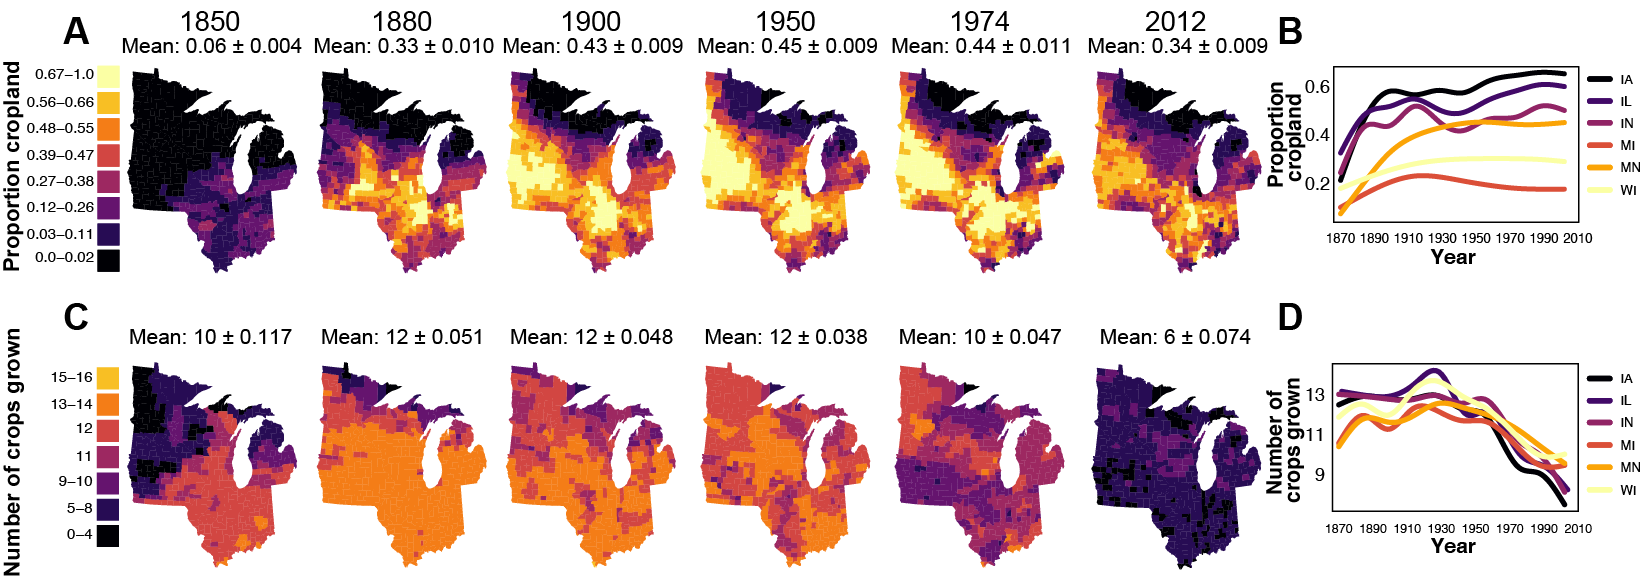
\includegraphics[width=1\textwidth,height=\textheight]{../ms_figs/fig_1.png}
\textbf{Figure 1:} Patterns of agricultural intensification in two
metrics: (A, B) proportion of county under cultivation and (C, D) number
of crops grown per county. Inset graphs (B,D) depict general trend of
these variables for each state in the study area as modeled by a Loess
curve. \clearpage

\newpage

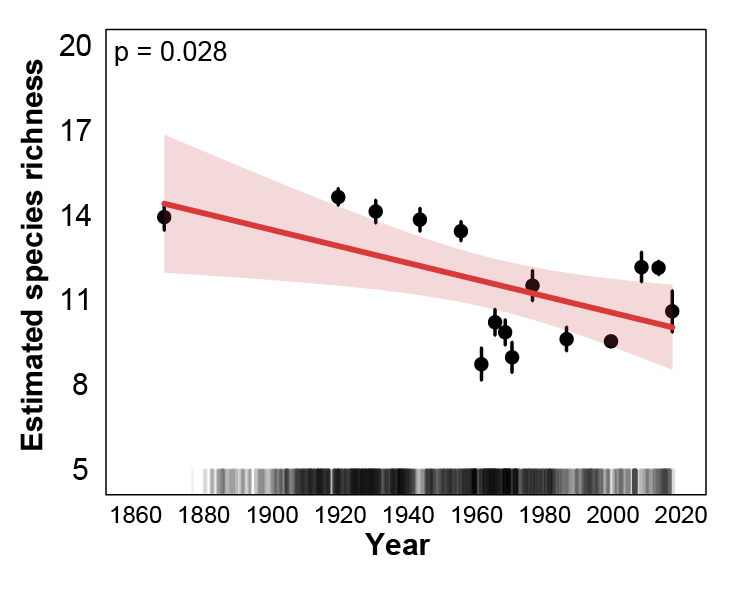
\includegraphics[width=1\textwidth,height=\textheight]{../ms_figs/fig_2.png}
\textbf{Figure 2:} Temporal trend of rarified bumble bee species
richness from 1877-present. Each point represents a date range that is
standardized to contain an approximately equal number of bumble bee
records (thus the date range differs for each point), and it is plotted
at the midpoint year of the date range. Error bars are 95\% confidence
intervals. The fitted line is a linear model predicting estimated
species richness as a function of temporal bin order using the midpoint
of the temporal bin as the predictor. Carpet plot represents temporal
collection year for all records from 1877 to present. \clearpage

\newpage

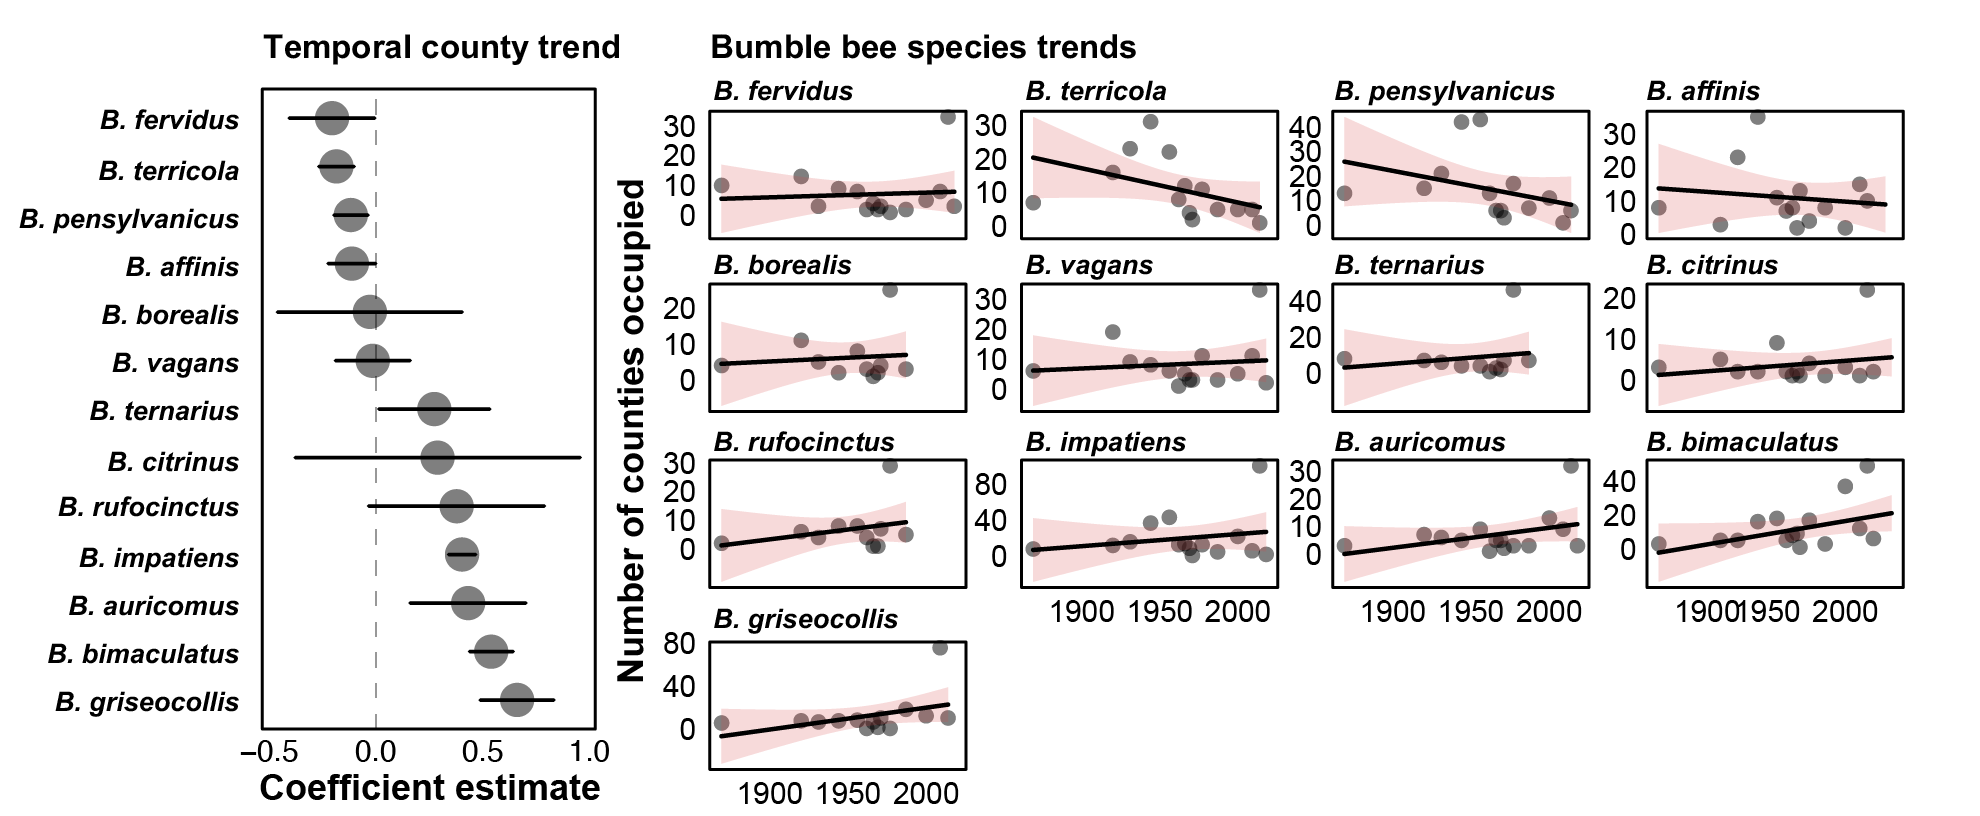
\includegraphics[width=1\textwidth,height=\textheight]{../ms_figs/fig_3.png}
\textbf{Figure 3:} Interaction plots for species of conservation concern
(first 3 rows) and common species (bottom 3 rows). Each line represents
the expected trend (with 95\% confidence interval) of probability of
occurrence over time in a county given: a value of proportion cropland
(panel columns: mean ± 1 standard deviation) and number of crops (line
color and type: mean ± 1 standard deviation) in that county. \clearpage

\newpage

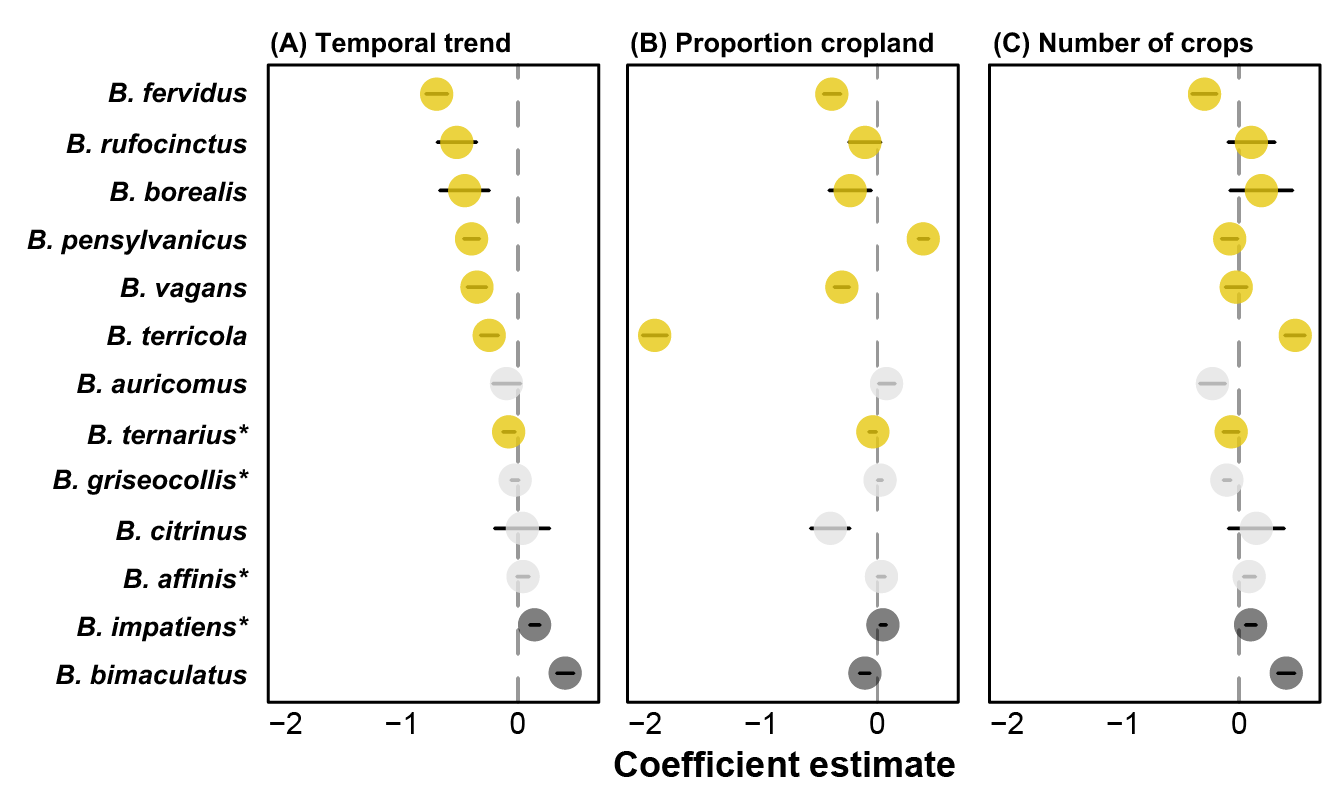
\includegraphics[width=1\textwidth,height=\textheight]{../ms_figs/fig_4.png}
\textbf{Figure 5:} (A) Predicted probability of occurrence for each
county within the study region from red (less likely) to green (more
likely). (B) Overall likelihood of occurrence over time from black (less
likely) to yellow (more likely). County values reflect quantile binned
slope coefficient estimates from a linear model predicting county
probability over occurrence 19 agricultural census time points. (C)
Predicted temporal trend in probability of occurrence across all
counties given agricultural conditions in each county . Each point is a
single county x year (jittered slightly for visibility), with a random
subset of 1000 points plotted (out of \textasciitilde{}11,000 total).
Temporal trend line is a simple generalized additive model to visualize
trend. All predictions generated using county-level agricultural
statistics and models (equation 1) fit for each species. \clearpage

\newpage

\hypertarget{supplementary-materials}{%
\section{Supplementary Materials}\label{supplementary-materials}}

\textbf{Table S1:} Generalized linear model results for each study
species (model equation 1) including the model type, sample size (number
of counties for which relative abundance is calculated), Moran I p-vale
(for Spatial error model types only), model McFadden Pseudo coefficient
of determination, model term, scaled coefficient estimate, 95\%
confidence interval and p-value. Each county is weighted by the total
number of bumble bee records for a given time point (agricultural census
year).
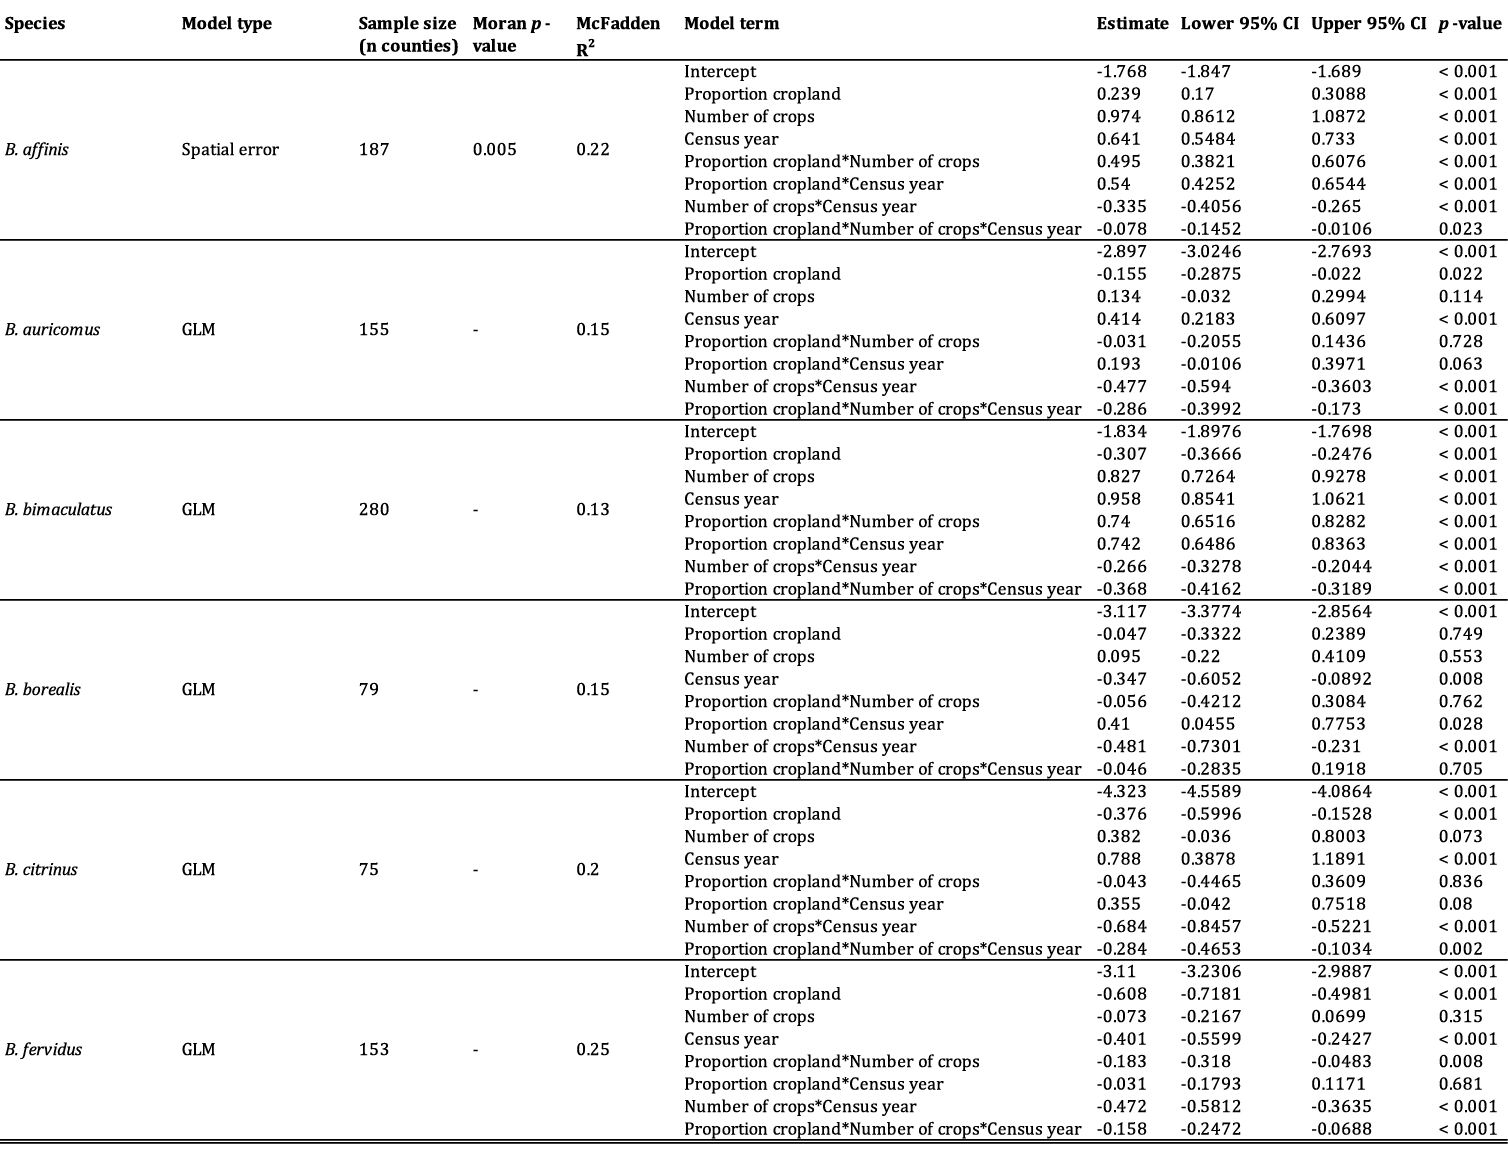
\includegraphics[width=1\textwidth,height=\textheight]{../ms_figs/table_s1_a.png}
\clearpage

\newpage

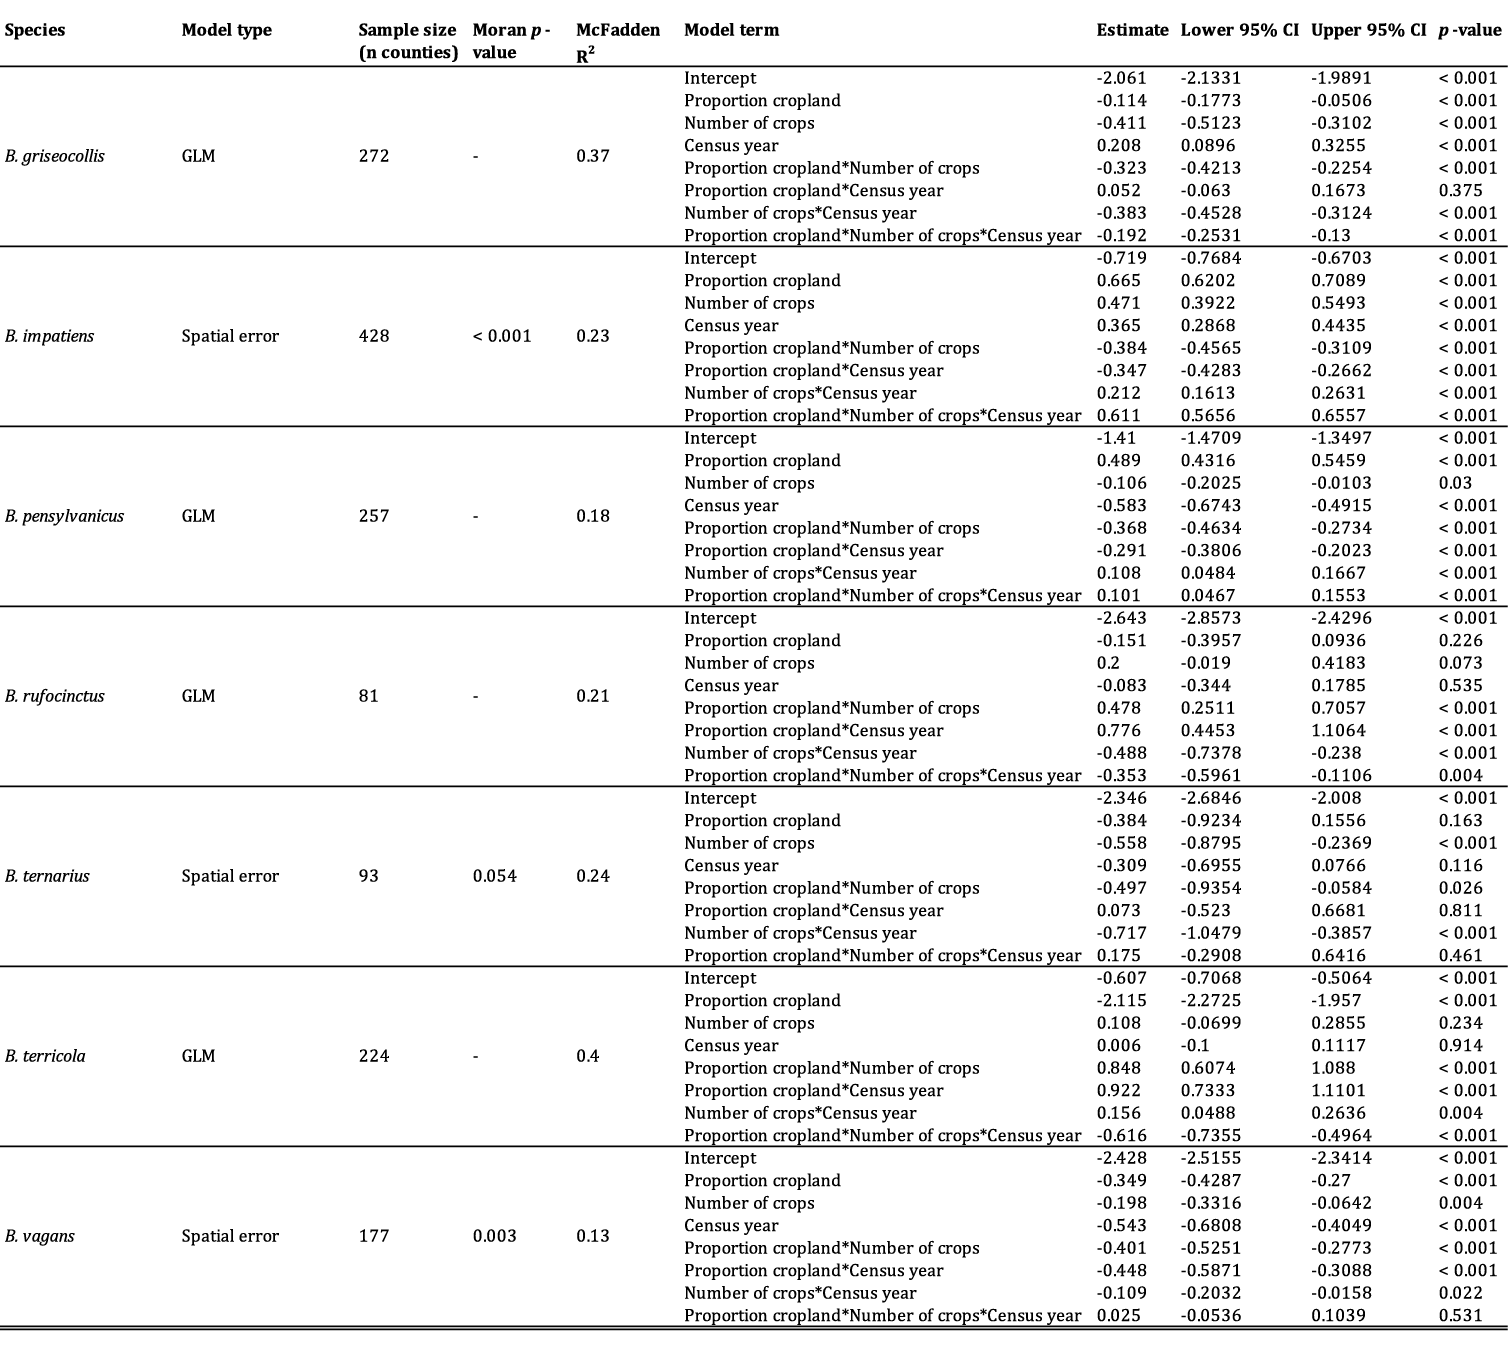
\includegraphics[width=1\textwidth,height=\textheight]{../ms_figs/table_s1_b.png}

\newpage

\textbf{Table S1:} Generalized linear model results for each study
species (model equation 2) including the model type, sample size (number
of counties for which relative abundance is calculated), Moran I p-vale
(for Spatial error model types only), model McFadden Pseudo coefficient
of determination, model term, scaled coefficient estimate, 95\%
confidence interval and p-value. Each county is weighted by the total
number of bumble bee records for a given time point (agricultural census
year).
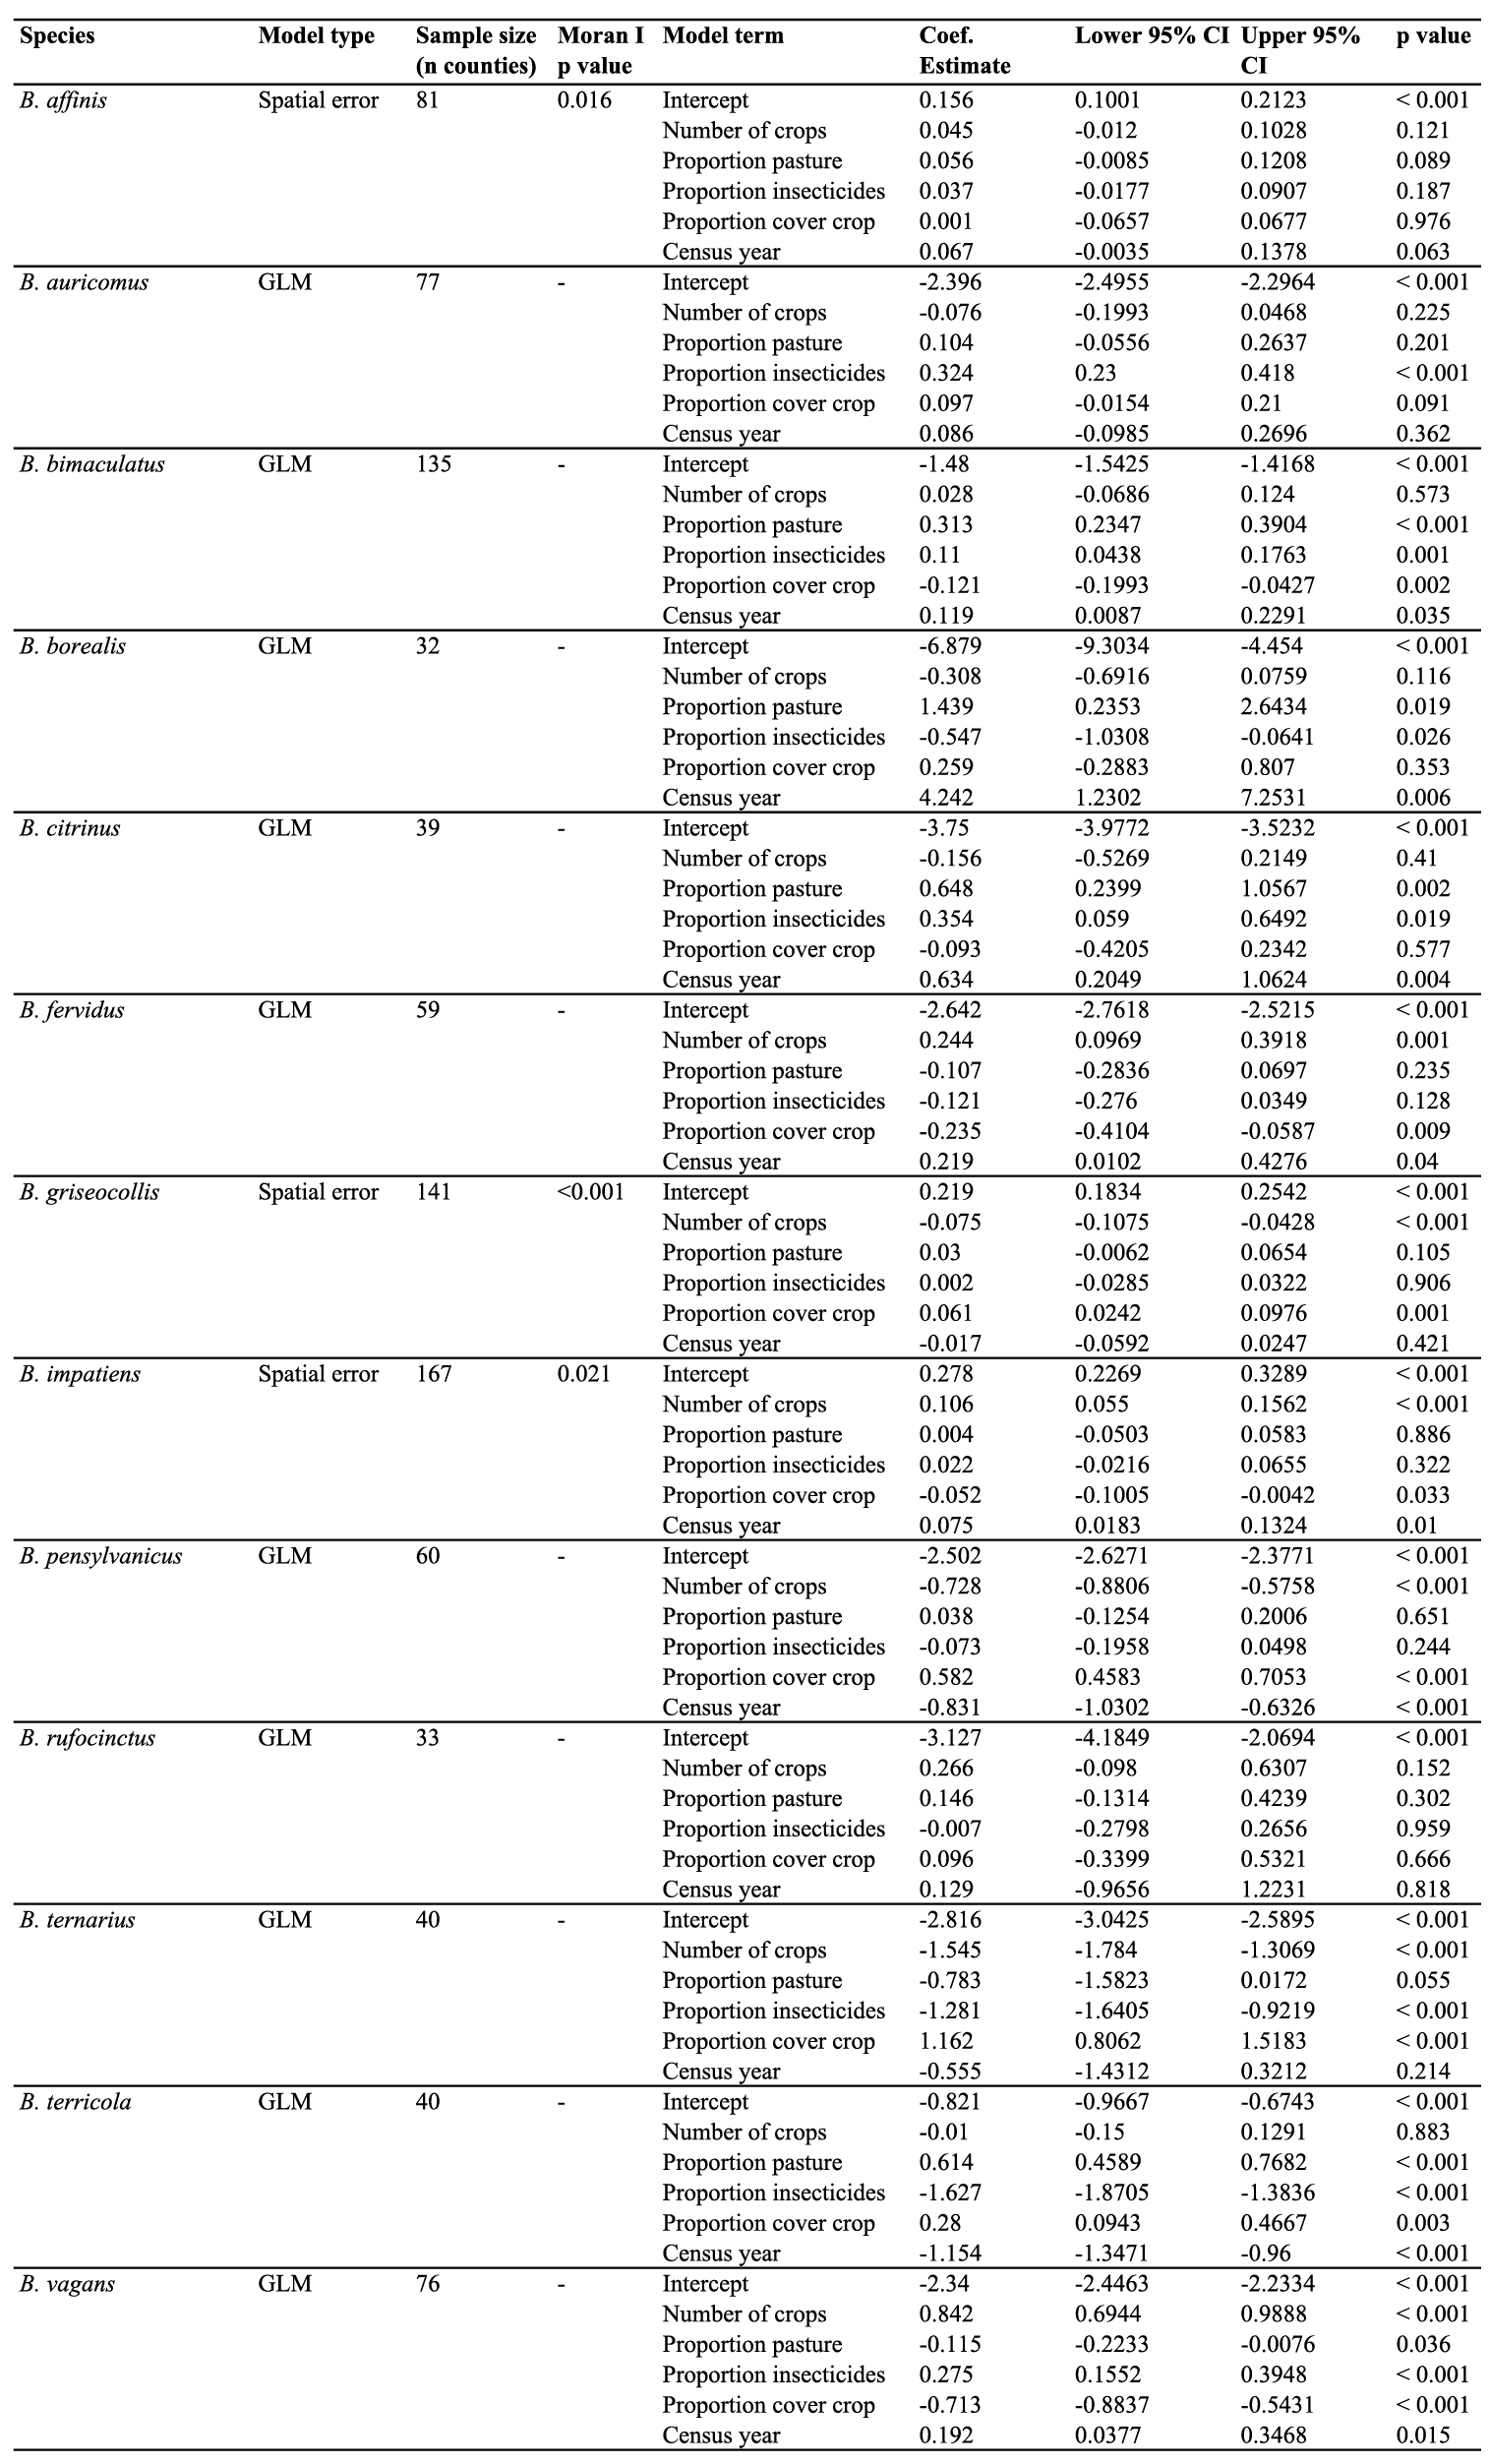
\includegraphics[width=1\textwidth,height=\textheight]{../ms_figs/table_s2.png}
\clearpage

\newpage

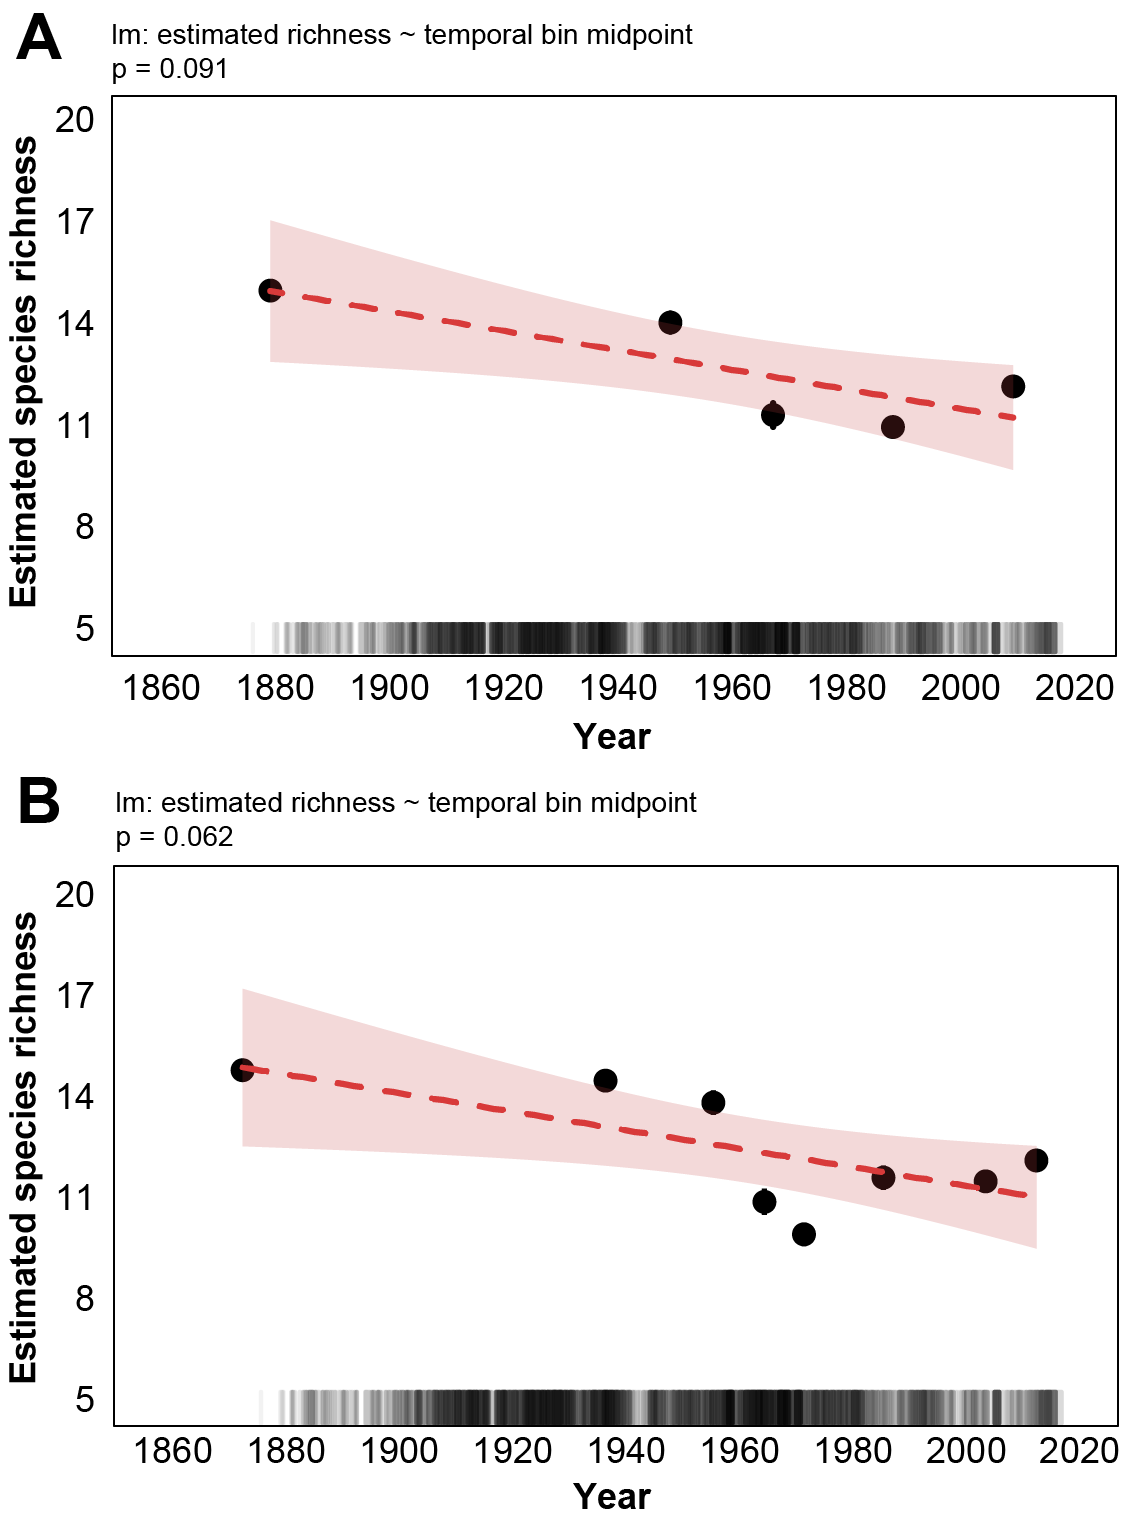
\includegraphics[width=1\textwidth,height=\textheight]{../ms_figs/fig_s1.png}
\textbf{Figure S1:} Patterns of agricultural intensification in two
additional metrics from 1982-2012: (A) proportion of county area in
pasture and (C) proportion of county area treated with insecticides.
Color palettes derived using quantile binning. Inset graphs (B,D) depict
general trend of these two variables for each state in the study area as
modeled by a Loess curve. Values beneath years are mean proportion ±
SEM. \clearpage

\newpage

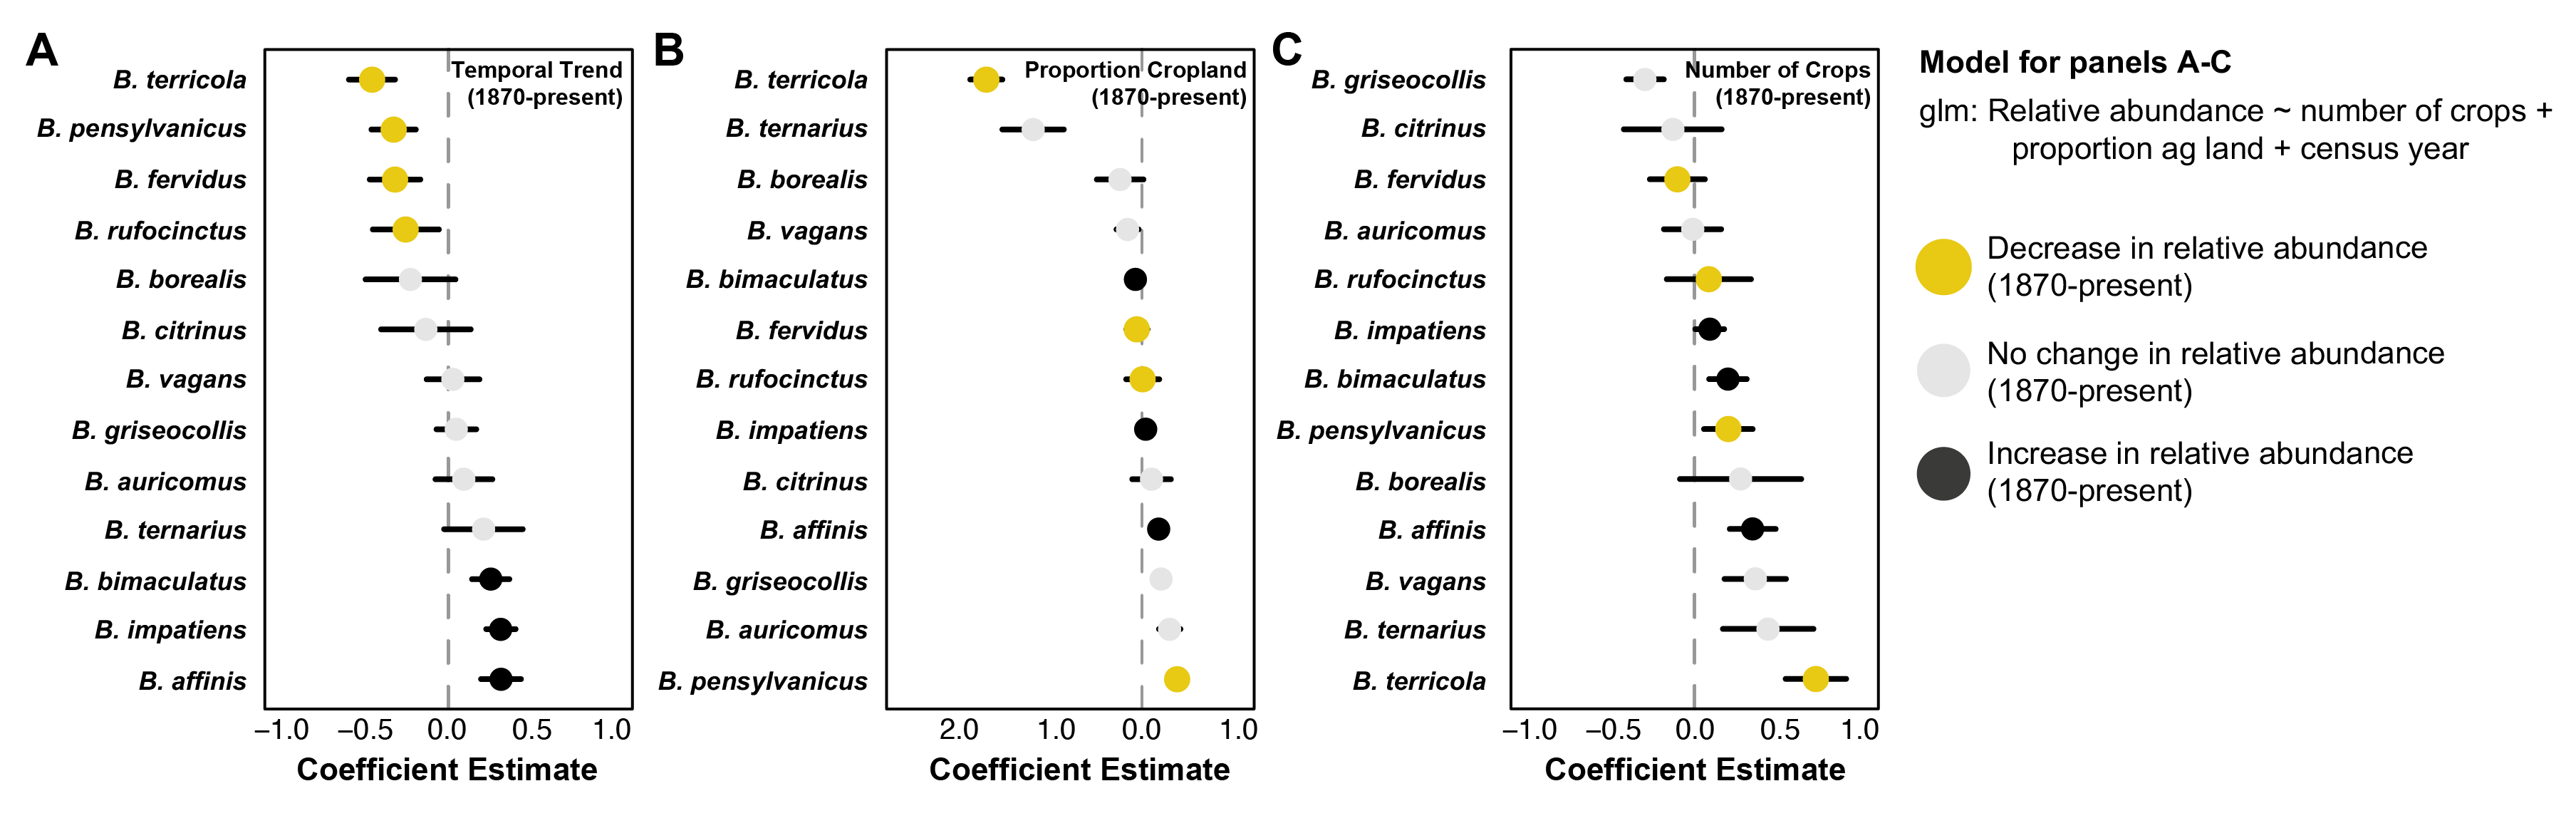
\includegraphics[width=1\textwidth,height=\textheight]{../ms_figs/fig_s2.png}
\textbf{Figure S2:} Interaction plots for other study species. Each line
represents the expected trend (with 95\% confidence interval) of
probability of occurrence over time in a county given: a value of
proportion cropland (panel columns: mean ± 1 standard deviation) and
number of crops (line color and type: mean ± 1 standard deviation) in
that county. \clearpage

\newpage

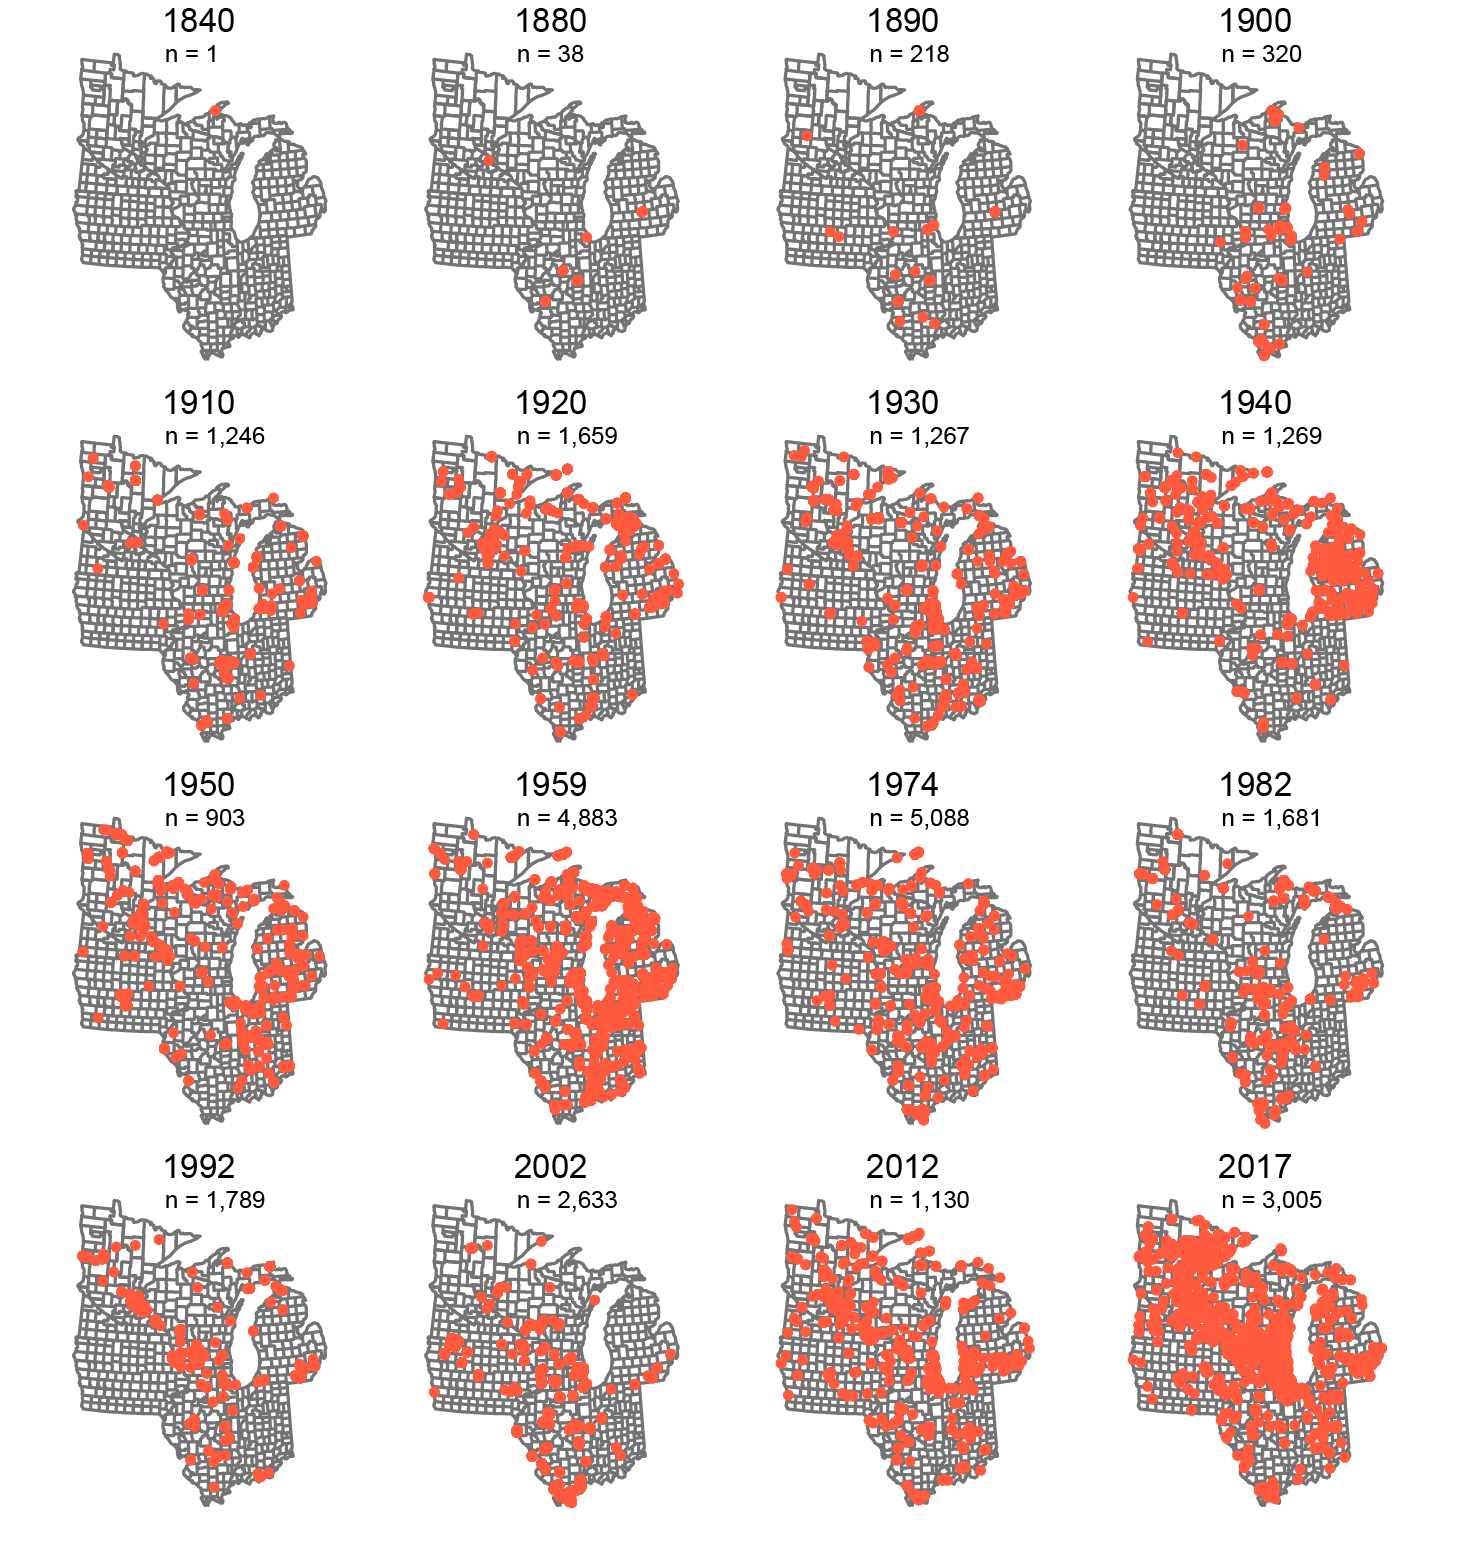
\includegraphics[width=1\textwidth,height=\textheight]{../ms_figs/fig_s3.png}
\textbf{Figure S3:} (A) Predicted probability of occurrence for each
county within the study region from red (less likely) to green (more
likely). (B) Overall likelihood of occurrence over time from black (less
likely) to yellow (more likely). County values reflect quantile binned
slope coefficient estimates from a linear model predicting county
probability over occurrence 19 agricultural census time points. (C)
Predicted temporal trend in probability of occurrence across all
counties given agricultural conditions in each county . Each point is a
single county x year (jittered slightly for visibility), with a random
subset of 1000 points plotted (out of \textasciitilde{}11,000 total).
Temporal trend line is a simple generalized additive model to visualize
trend. All predictions generated using county-level agricultural
statistics and models (equation 1) fit for each species. \clearpage

\newpage

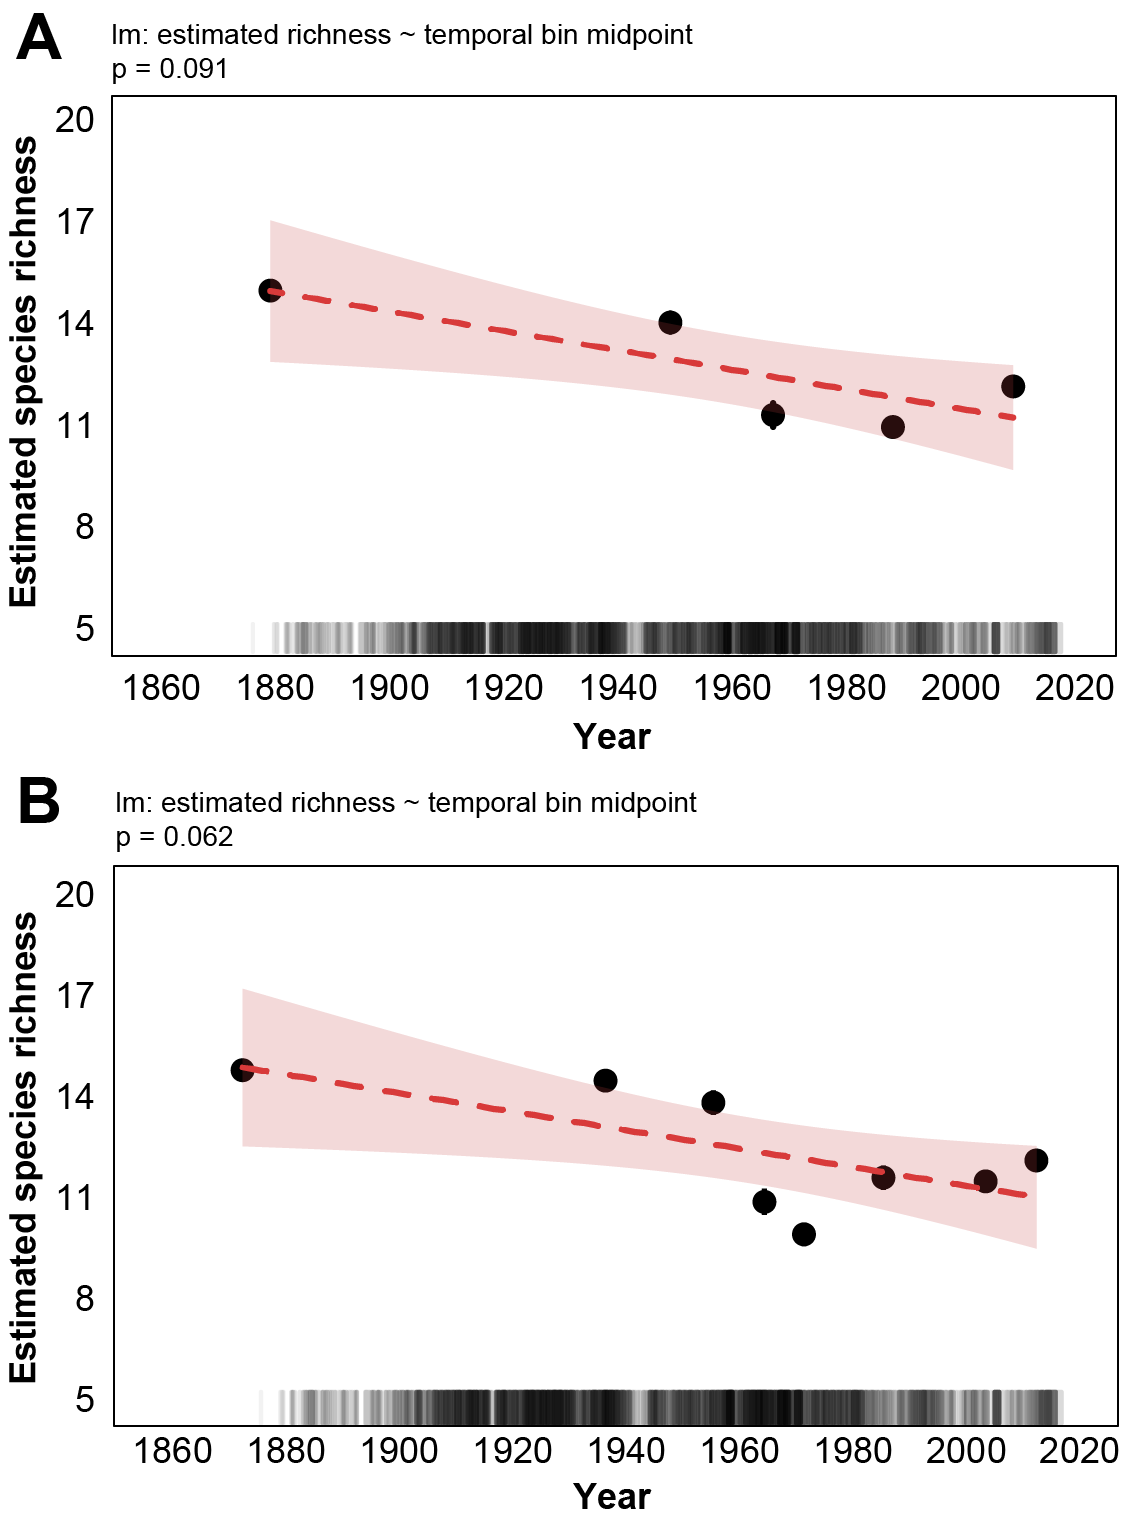
\includegraphics[width=1\textwidth,height=\textheight]{../ms_figs/fig_s4.png}
\textbf{Figure S4:} The relative proportion of county area of the 18
crop types included within the study from 1840-2017. Other category
includes 13 crops that together compose less than 5\% of county area at
any time point. \clearpage

\newpage

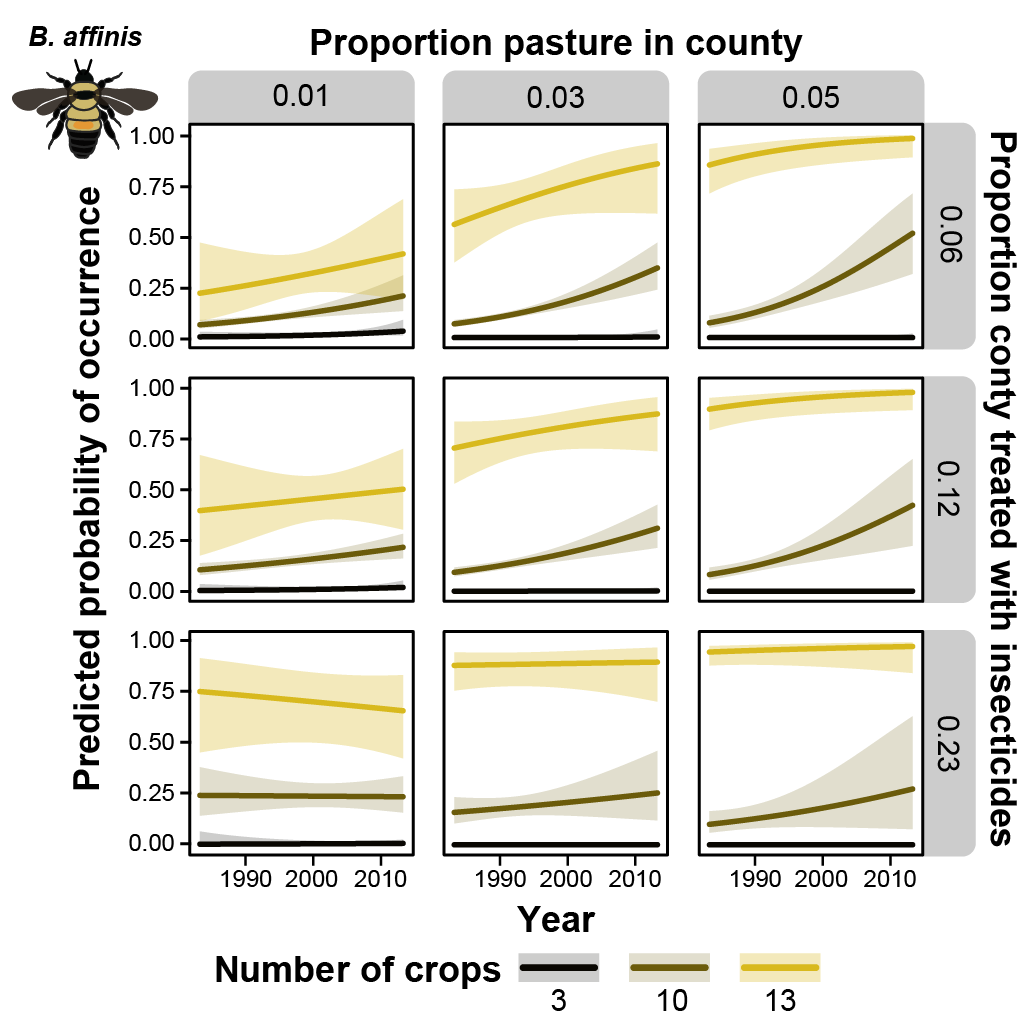
\includegraphics[width=1\textwidth,height=\textheight]{../ms_figs/fig_s5.png}
\textbf{Figure S5:} Interaction plots for \emph{B. affinis}. Each line
represents the expected trend (with 95\% confidence interval) of
probability of occurrence over time in a county given: a value of
proportion pasture (panel columns: mean ± 1 standard deviation),
proportion of county treated with insecticides (panel rows: mean ± 1
standard deviation) and number of crops (line color and type: mean ± 1
standard deviation) in that county. \clearpage

\newpage

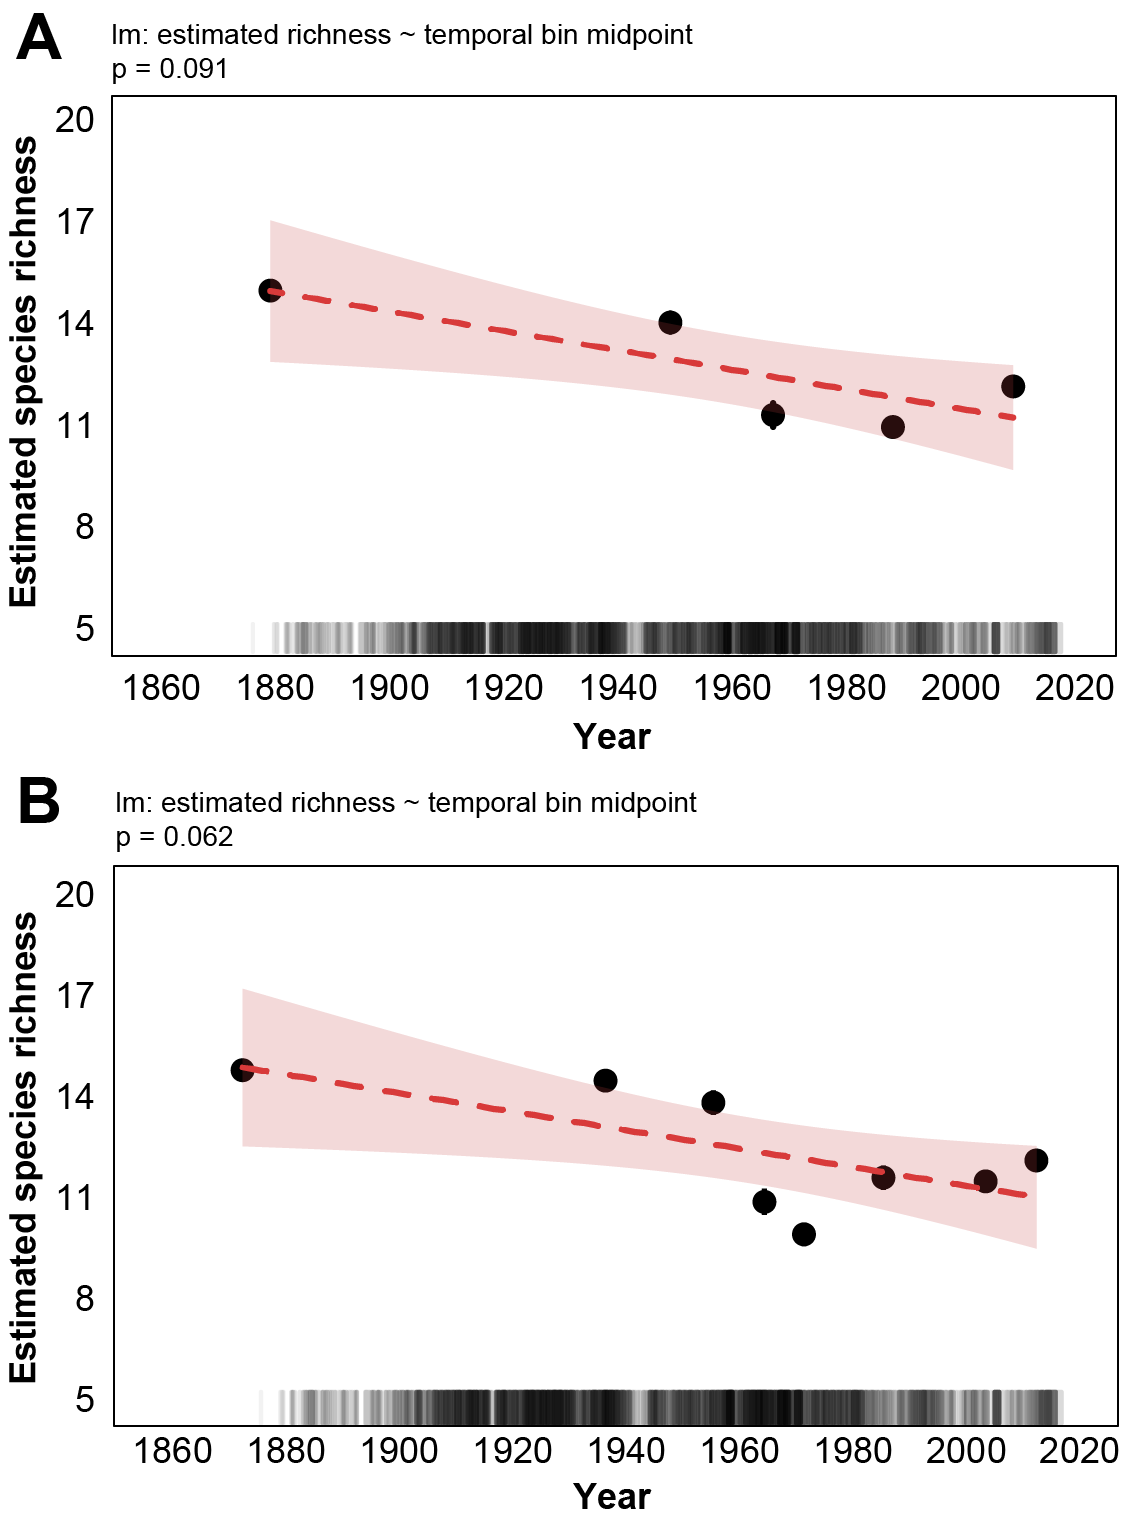
\includegraphics[width=1\textwidth,height=\textheight]{../ms_figs/fig_s6.png}
\textbf{Figure S6:} Interaction plots for \emph{B. pensylvanicus}. Each
line represents the expected trend (with 95\% confidence interval) of
probability of occurrence over time in a county given: a value of
proportion pasture (panel columns: mean ± 1 standard deviation),
proportion of county treated with insecticides (panel rows: mean ± 1
standard deviation) and number of crops (line color and type: mean ± 1
standard deviation) in that county. \clearpage

\newpage

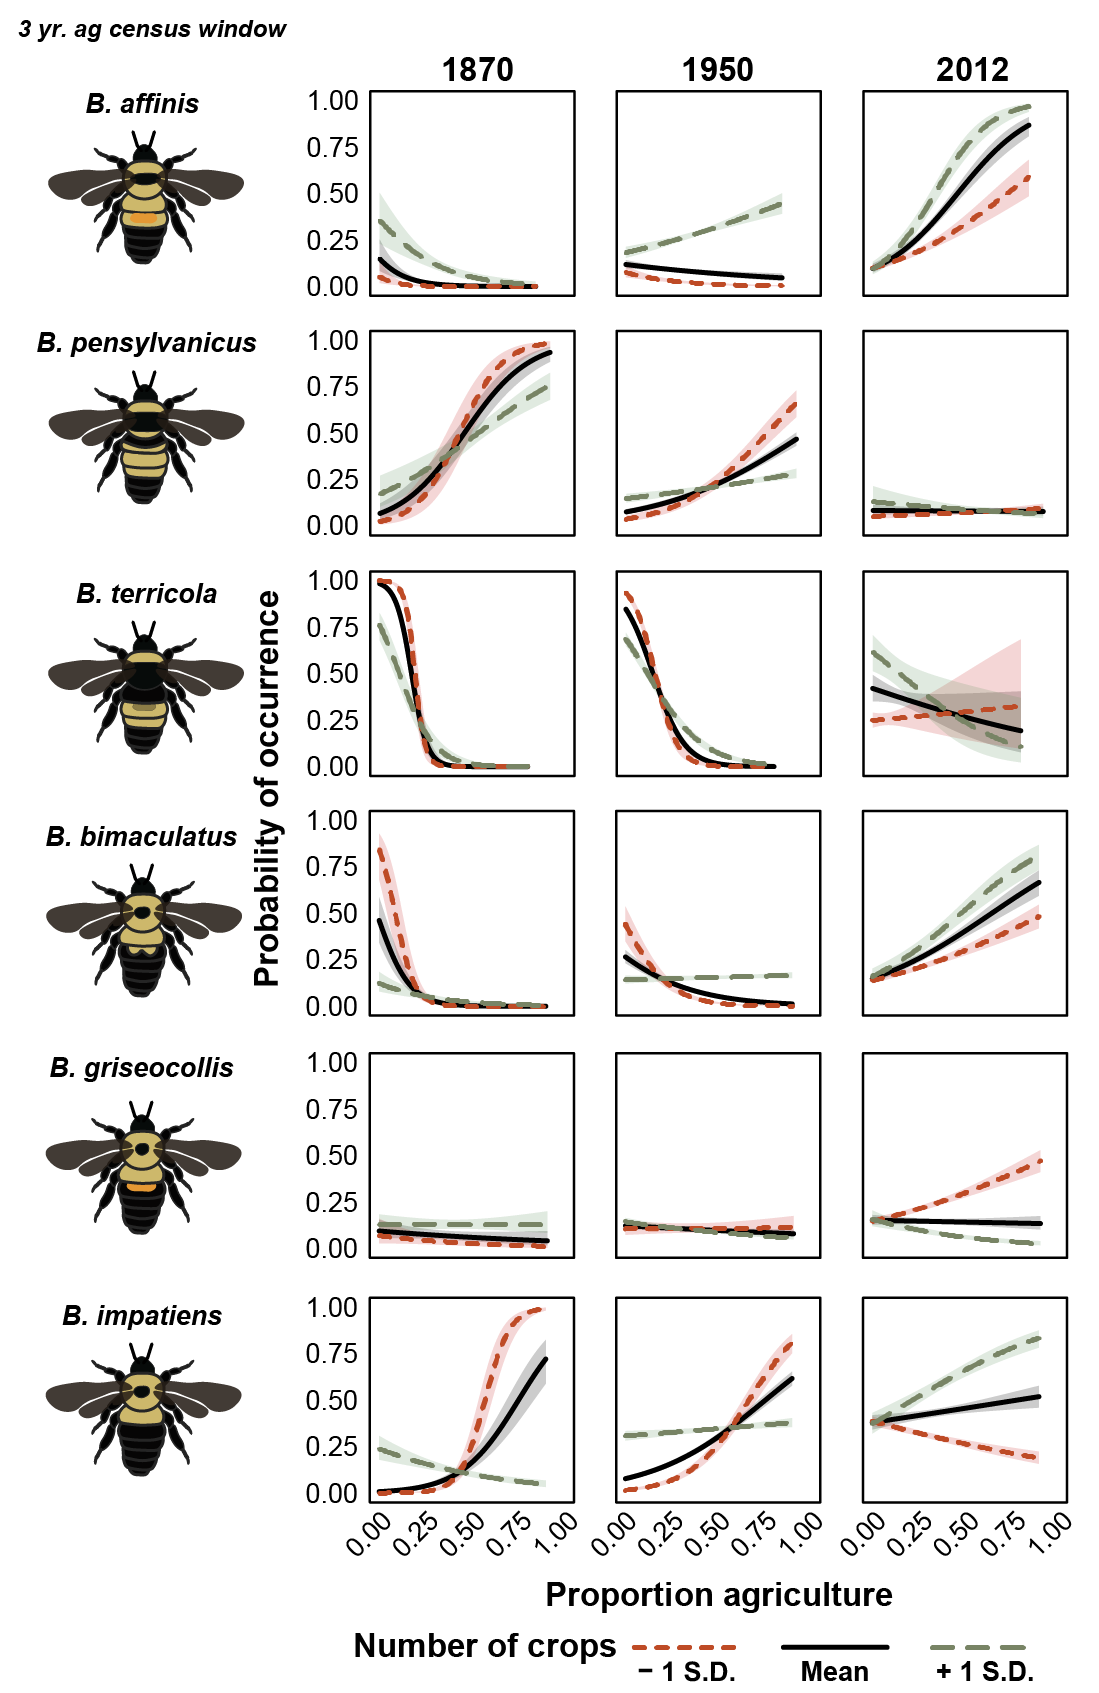
\includegraphics[width=1\textwidth,height=\textheight]{../ms_figs/fig_s7.png}
\textbf{Figure S7:} Interaction plots for \emph{B. terricola}. Each line
represents the expected trend (with 95\% confidence interval) of
probability of occurrence over time in a county given: a value of
proportion pasture (panel columns: mean ± 1 standard deviation),
proportion of county treated with insecticides (panel rows: mean ± 1
standard deviation) and number of crops (line color and type: mean ± 1
standard deviation) in that county. \clearpage

\newpage

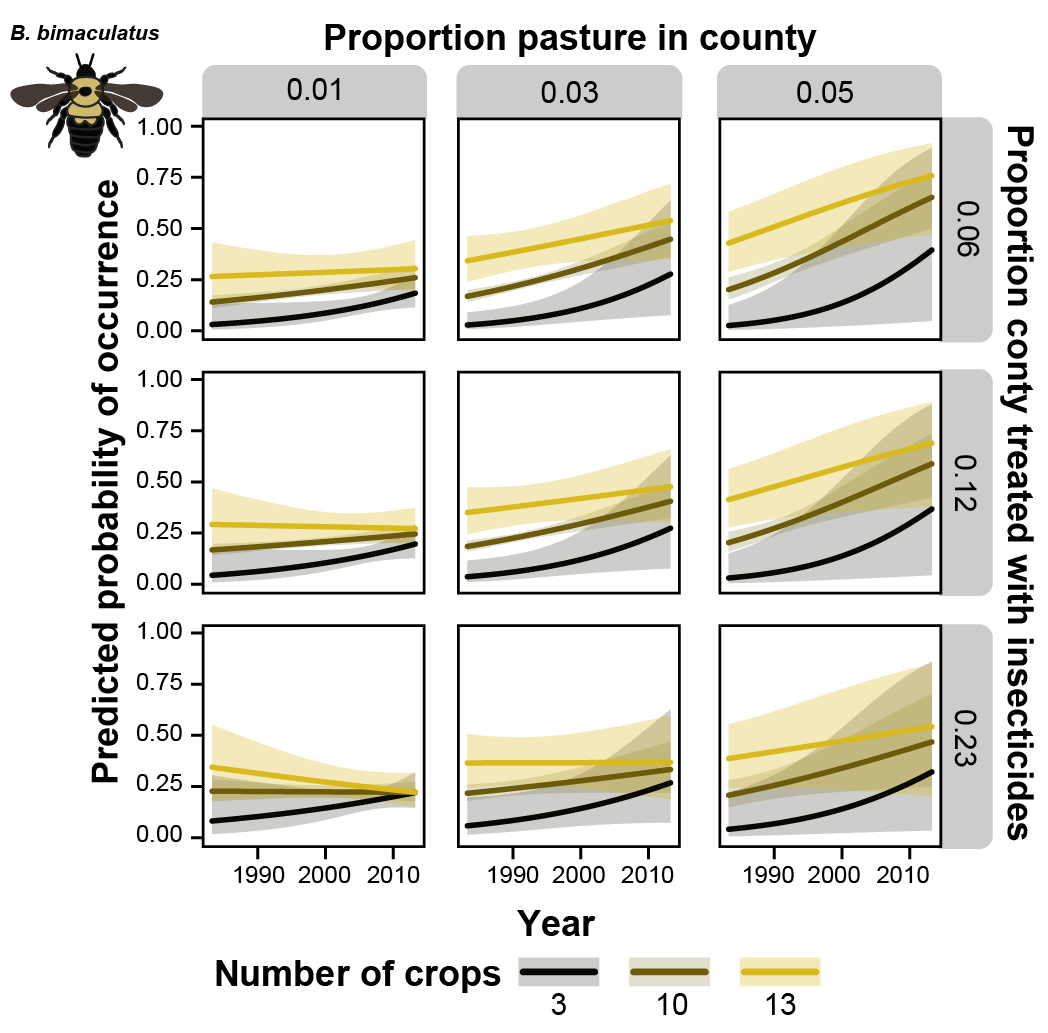
\includegraphics[width=1\textwidth,height=\textheight]{../ms_figs/fig_s8.png}
\textbf{Figure S8:} Interaction plots for \emph{B. bimaculatus}. Each
line represents the expected trend (with 95\% confidence interval) of
probability of occurrence over time in a county given: a value of
proportion pasture (panel columns: mean ± 1 standard deviation),
proportion of county treated with insecticides (panel rows: mean ± 1
standard deviation) and number of crops (line color and type: mean ± 1
standard deviation) in that county. \clearpage

\newpage

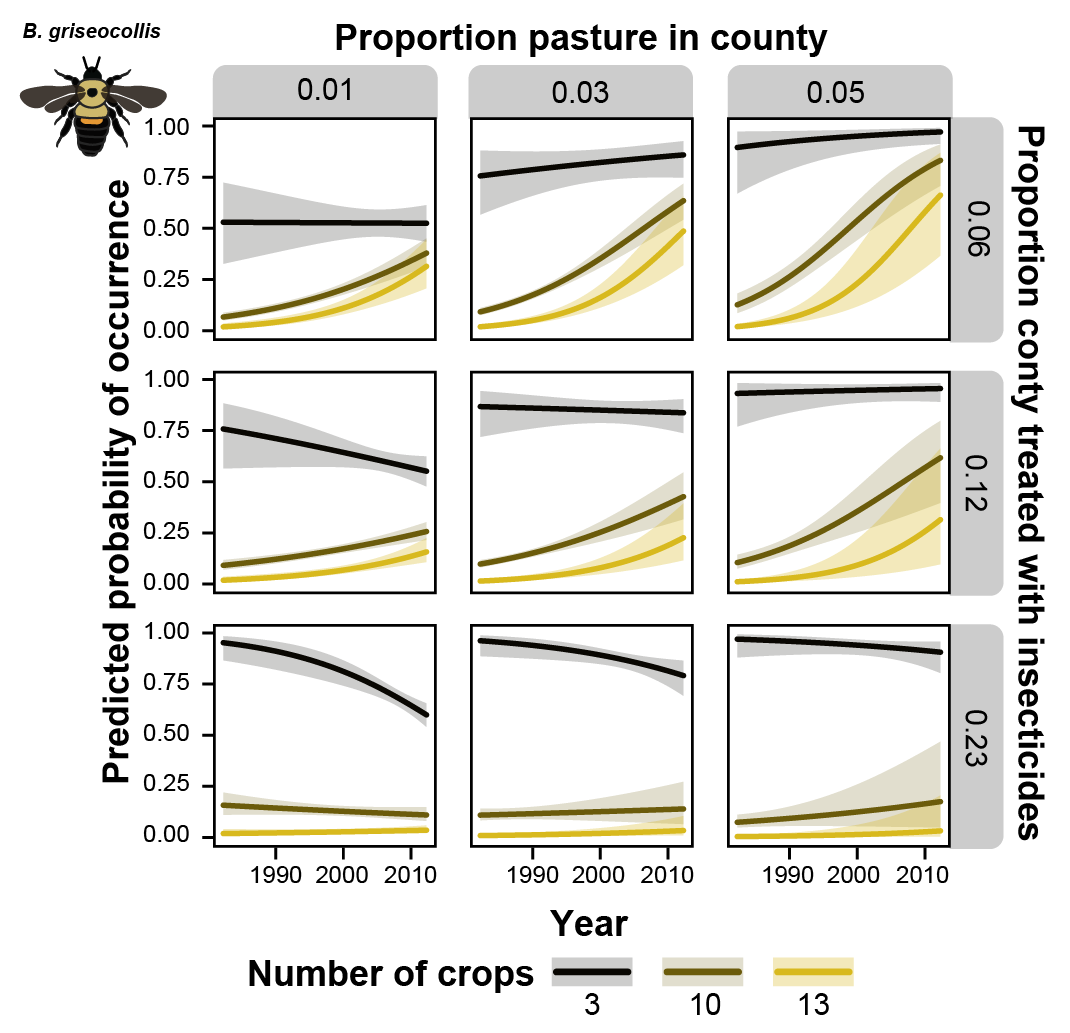
\includegraphics[width=1\textwidth,height=\textheight]{../ms_figs/fig_s9.png}
\textbf{Figure S9:} Interaction plots for \emph{B. griseocollis}. Each
line represents the expected trend (with 95\% confidence interval) of
probability of occurrence over time in a county given: a value of
proportion pasture (panel columns: mean ± 1 standard deviation),
proportion of county treated with insecticides (panel rows: mean ± 1
standard deviation) and number of crops (line color and type: mean ± 1
standard deviation) in that county. \clearpage

\newpage

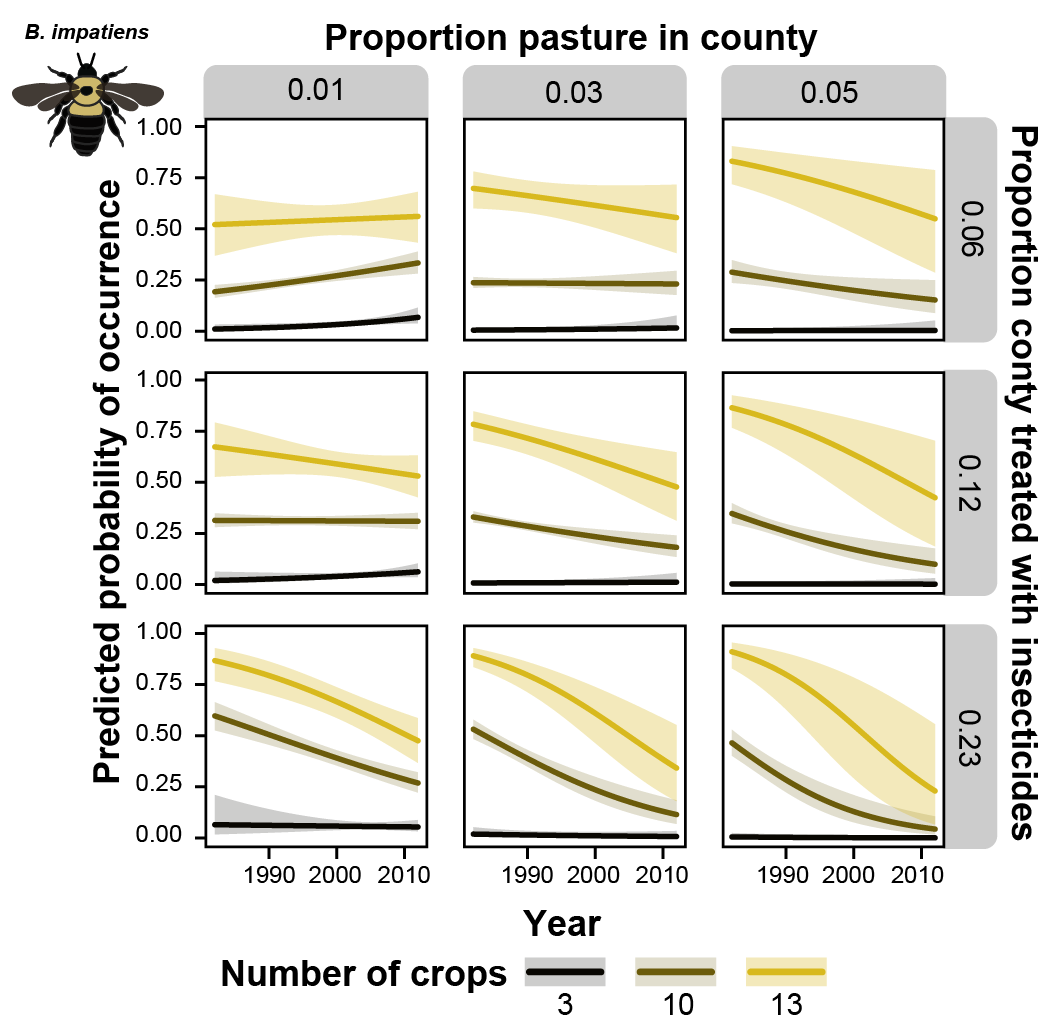
\includegraphics[width=1\textwidth,height=\textheight]{../ms_figs/fig_s10.png}
\textbf{Figure S10:} Interaction plots for \emph{B. impatiens}. Each
line represents the expected trend (with 95\% confidence interval) of
probability of occurrence over time in a county given: a value of
proportion pasture (panel columns: mean ± 1 standard deviation),
proportion of county treated with insecticides (panel rows: mean ± 1
standard deviation) and number of crops (line color and type: mean ± 1
standard deviation) in that county. \clearpage

\newpage

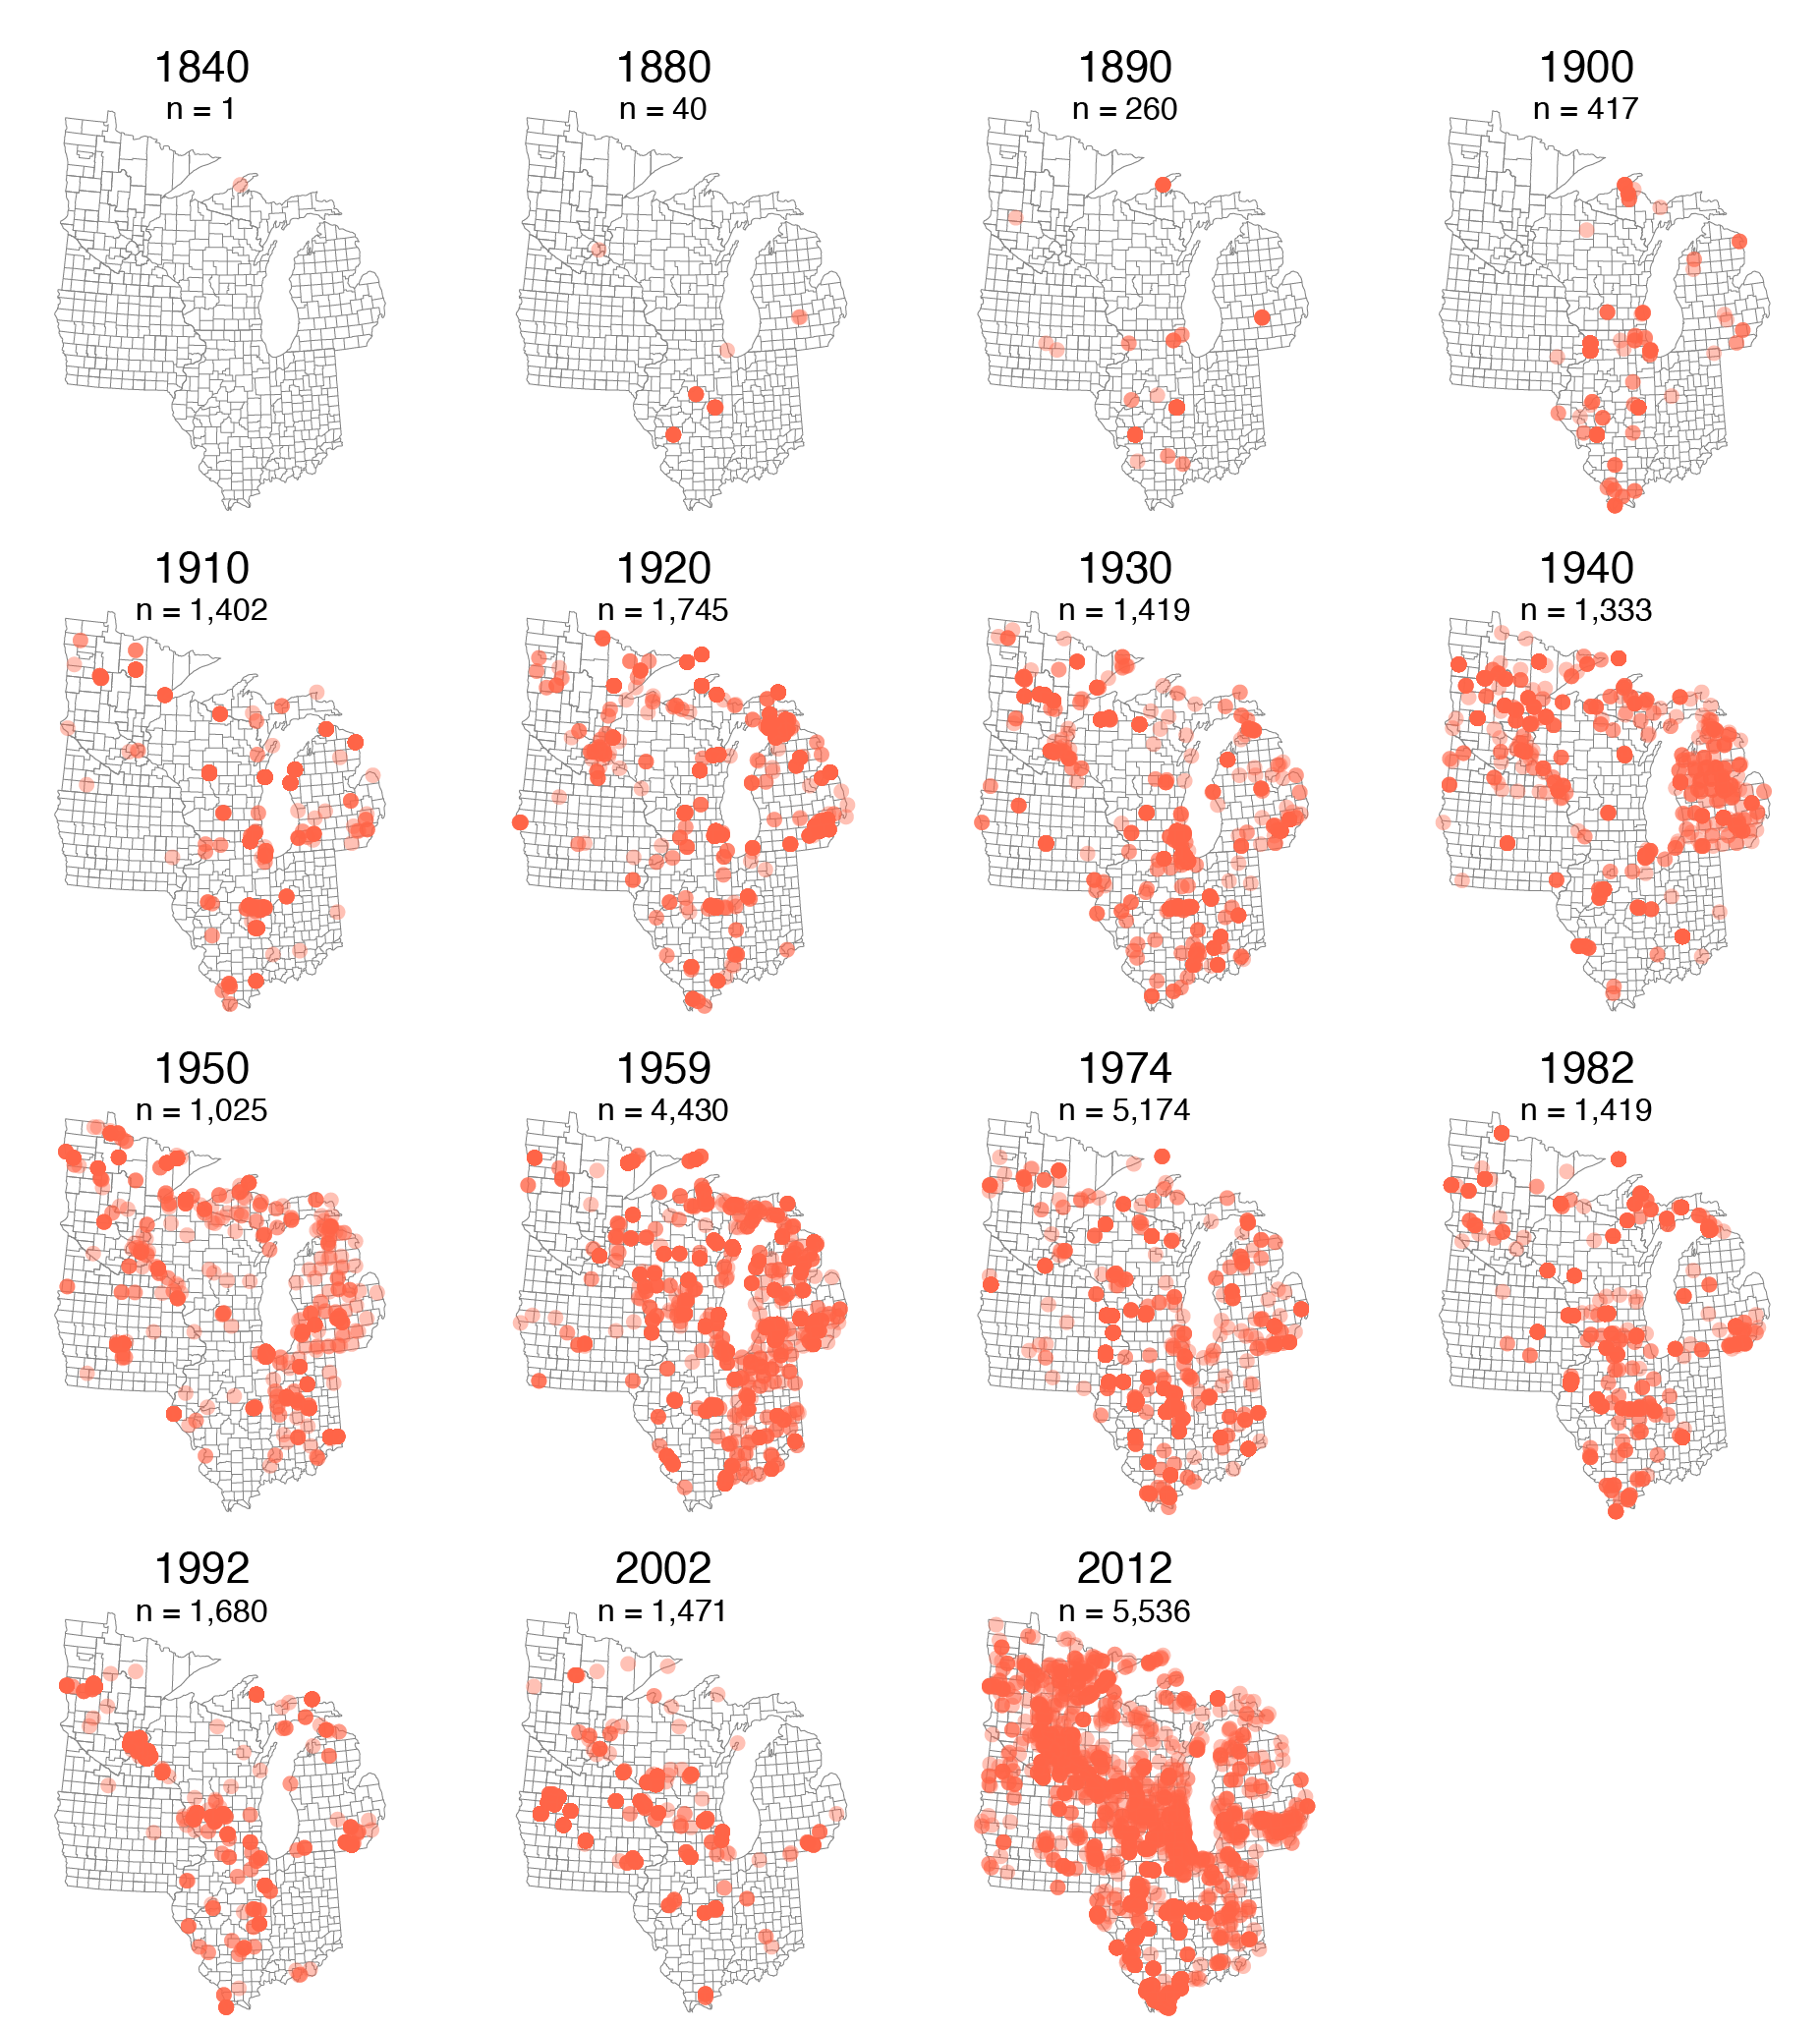
\includegraphics[width=1\textwidth,height=\textheight]{../ms_figs/fig_s11.png}
\textbf{Figure S11:} The location of bumble bee records binned from ±5
years of each US Census of Agriculture year considered in our analysis.
The number of records is noted below the year. Points are partially
transparent and jittered slightly for visibility. \clearpage

\newpage

\textbf{Analysis filtering data to unique species x location x collector
x date combinations} To determine whether sampling effort by individuals
skewed the results of our analysis, we fit our primary model (relative
abundance \textasciitilde{} proportion cropland + number of crops +
agricultural census year; results shown in Fig. 5) to a reduced dataset,
filtering records to include only unique combinations of species,
location, collector, and collection date. We found similar results in
the trend and statistical effect of each interaction.

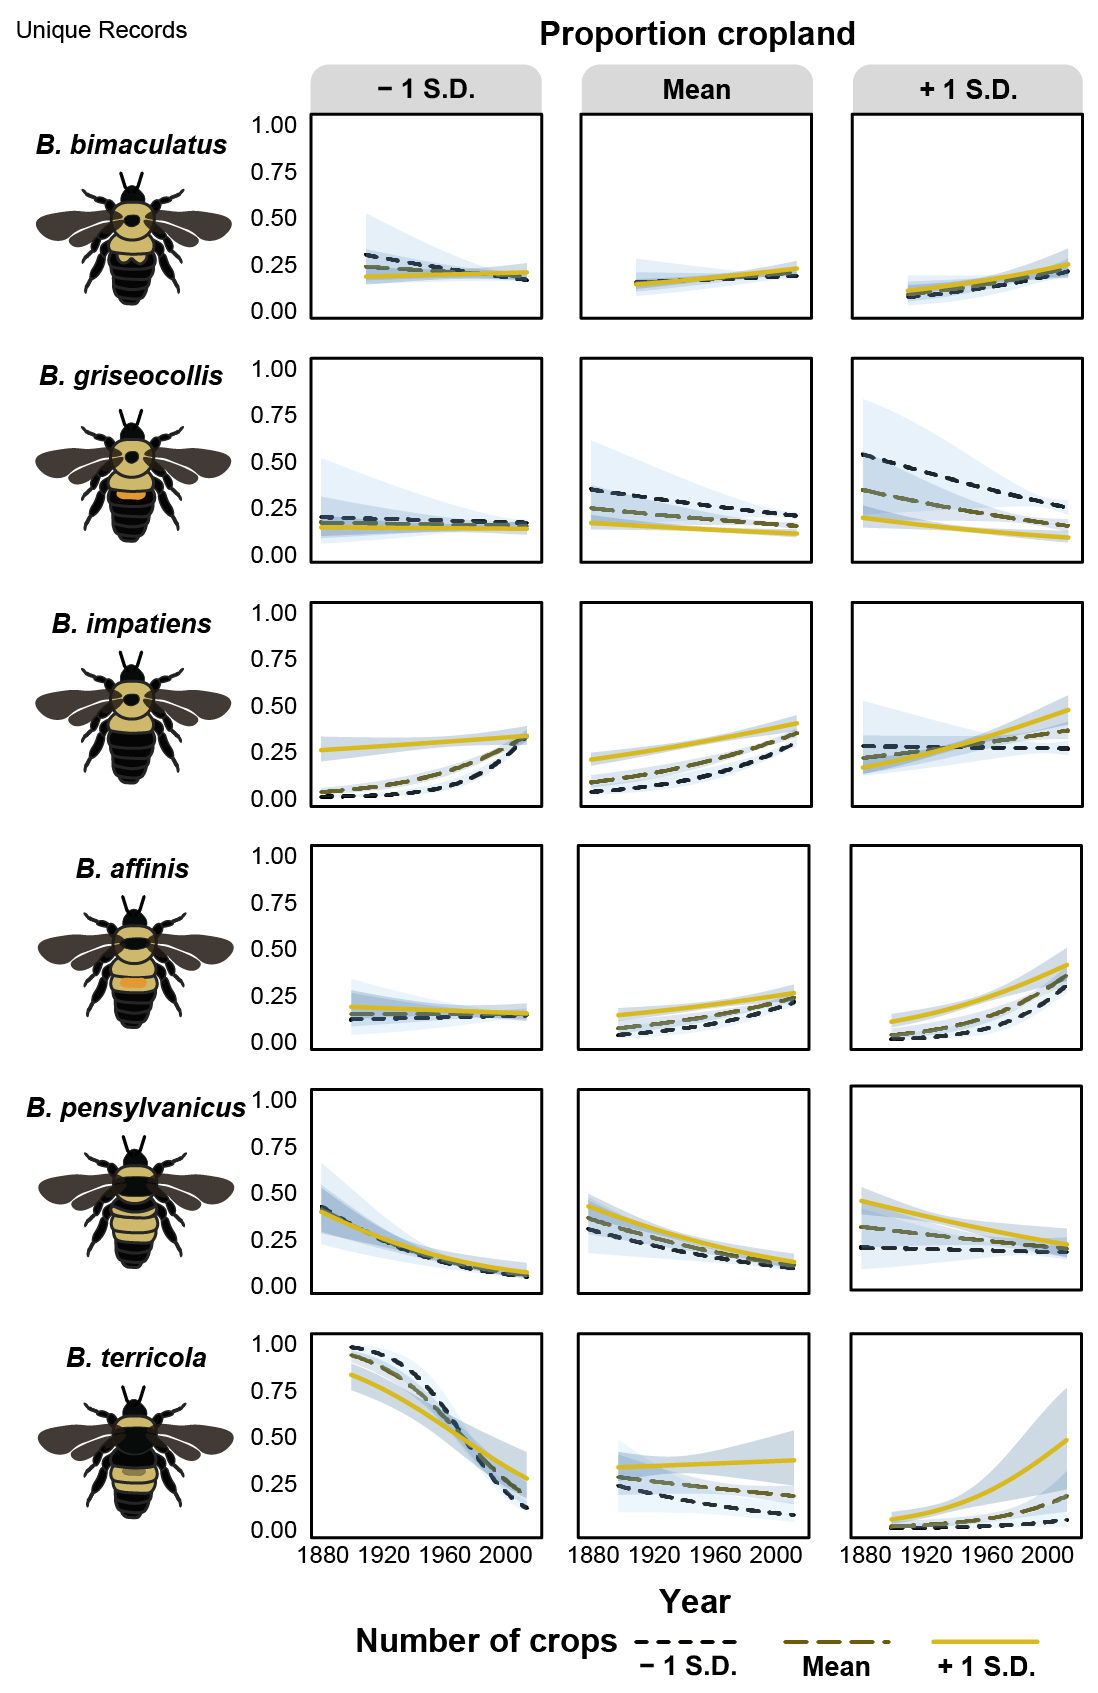
\includegraphics[width=1\textwidth,height=\textheight]{../ms_figs/fig_s12.png}
\textbf{Figure S12:} Interaction plots for species of conservation
concern (first three rows) and common species (last 3 rows). Each line
represents the expected trend (with 95\% confidence interval) of
probability of occurrence over time in a county given: a value of
proportion cropland (panel columns: mean ± 1 standard deviation) and
number of crops (line color and type: mean ± 1 standard deviation) in
that county. \clearpage

\newpage

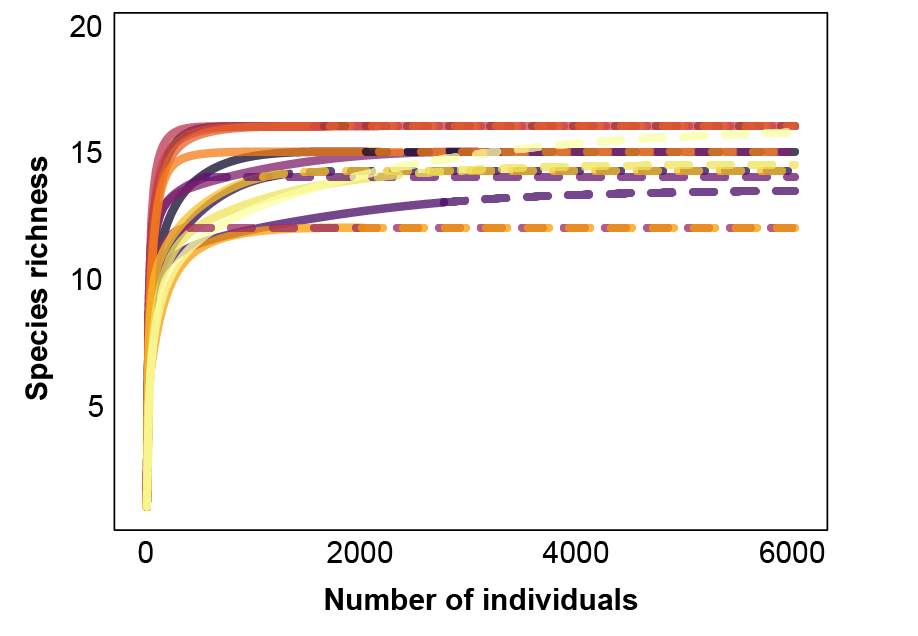
\includegraphics[width=1\textwidth,height=\textheight]{../ms_figs/fig_s13.png}
\textbf{Figure S13:} Sample-based species accumulation curves for each
of 15 temporal bins (different colors) from which estimated species
richness was calculated (Fig. 2). Each accumulation curve is constructed
for temporal bins with a roughly equal number of records. Solid lines
are interpolated from data, while dashed lines are extrapolated to a
6,000 record limit. \clearpage

\newpage

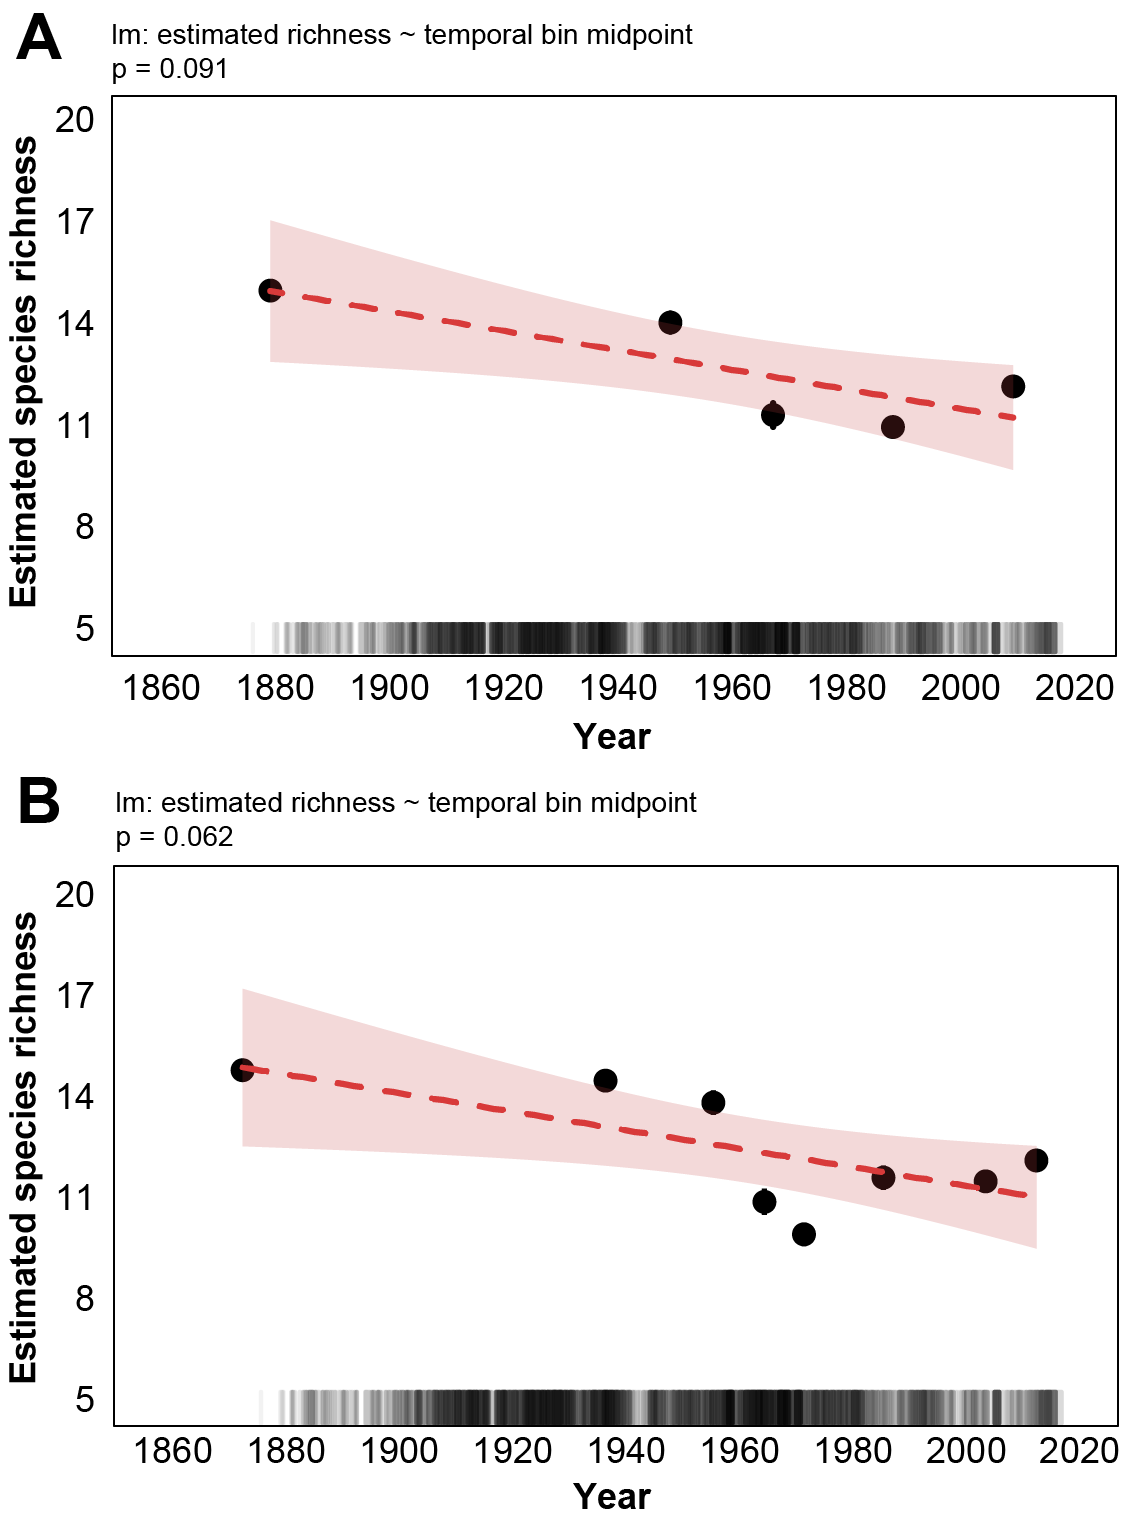
\includegraphics[width=1\textwidth,height=\textheight]{../ms_figs/fig_s14.png}
\textbf{Figure S14:} Trend in rarified bumble bee species richness from
1877-present for alternative numbers of temporal bins, each representing
approximately equal numbers of bumble bee records: (A) 5 temporal bins
and (B) 8 temporal bins. Each point is plotted at the midpoint of the
temporal bin date range. Error bars are 95\% confidence intervals. The
fitted line is a linear model predicting estimated species richness as a
function of temporal bin order using the midpoint year of the temporal
bin as the predictor. Carpet plot represents temporal collection year
for all records from 1877 to present. \clearpage

\newpage

\textbf{Analysis restricting to records within ± 3 years of agricultural
census} As agricultural census records are collected every 10 years, we
were required to pair bumble bee records to the nearest agricultural
census (a difference of up to ± 5 years). This requirement might skew
results if agricultural metrics display non-linear trends between census
years. To determine if this was the case, we filtered records such that
only bumble bee within ± 3 years of an agricultural census data were
included. Modeling these data resulted nearly identical interaction
patterns of predicted occurrence and agricultural metrics.

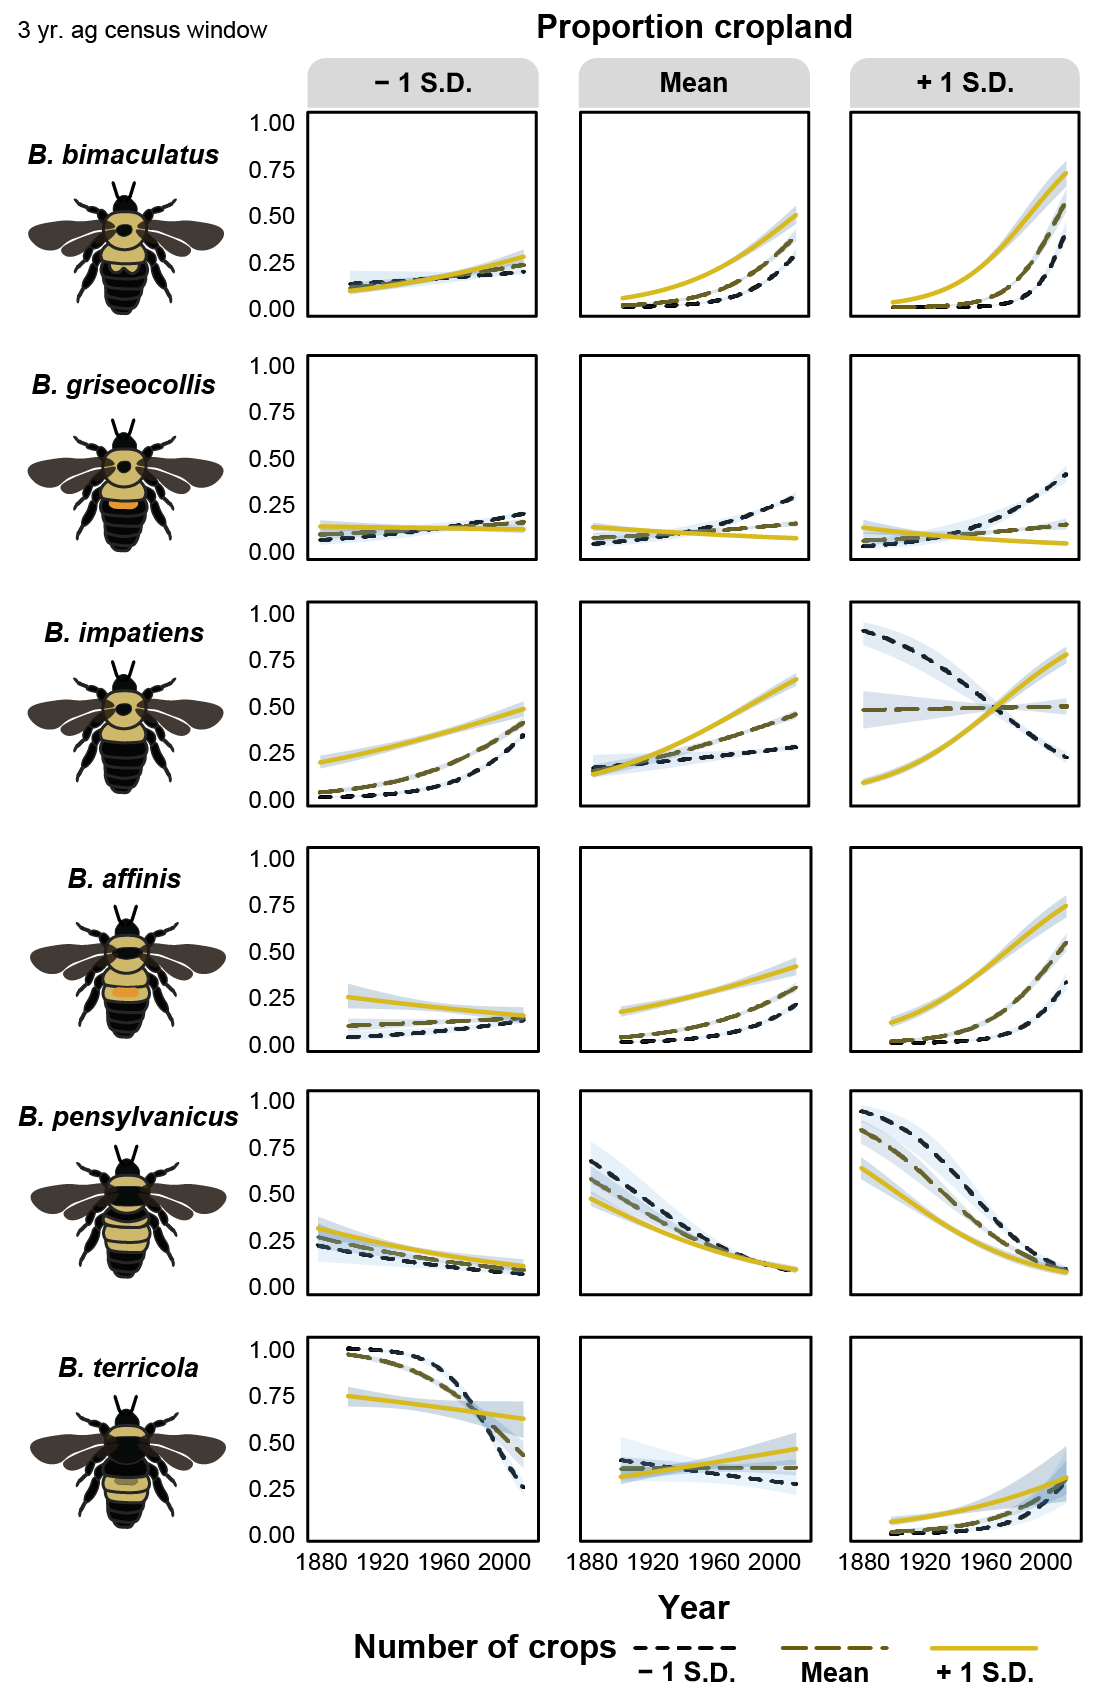
\includegraphics[width=1\textwidth,height=\textheight]{../ms_figs/fig_s15.png}
\textbf{Figure S15:} Interaction plots for species of conservation
concern (first three rows) and common species (last 3 rows). Each line
represents the expected trend (with 95\% confidence interval) of
probability of occurrence over time in a county given: a value of
proportion cropland (panel columns: mean ± 1 standard deviation) and
number of crops (line color and type: mean ± 1 standard deviation) in
that county. \clearpage

\hypertarget{references}{%
\section*{References}\label{references}}
\addcontentsline{toc}{section}{References}

\hypertarget{refs}{}
\leavevmode\hypertarget{ref-Bartomeus2019}{}%
Bartomeus I, Stavert JR, Ward D, Aguado O (2019) Historical collections
as a tool for assessing the global pollination crisis. Philos. Trans. R.
Soc. B Biol. Sci. 374: 1--9.
\url{https://doi.org/10.1098/rstb.2017.0389}

\leavevmode\hypertarget{ref-Bartomeus2013}{}%
Bartomeus I, Park MG, Gibbs J, Danforth BN, Lakso AN, Winfree R (2013)
Biodiversity ensures plant-pollinator phenological synchrony against
climate change. Ecol. Lett. 16: 1331--1338.
\url{https://doi.org/10.1111/ele.12170}

\leavevmode\hypertarget{ref-Benton2003}{}%
Benton TG, Vickery JA, Wilson JD (2003) Farmland biodiversity: Is
habitat heterogeneity the key? Trends Ecol. Evol. 18: 182--188.
\url{https://doi.org/10.1016/S0169-5347(03)00011-9}

\leavevmode\hypertarget{ref-Benton2002}{}%
Benton TG, Bryant DM, Cole L, Crick HQ (2002) Linking agricultural
practice to insect and bird populations: A historical study over three
decades. J. Appl. Ecol. 39: 673--687.
\url{https://doi.org/10.1046/j.1365-2664.2002.00745.x}

\leavevmode\hypertarget{ref-Biesmeijer2006}{}%
Biesmeijer JC (2006) Parallel Declines in Pollinators and
Insect-Pollinated Plants in Britain and the Netherlands. Science (80-.
). 313: 351--354. \url{https://doi.org/10.1126/science.1127863}

\leavevmode\hypertarget{ref-Brown2011}{}%
Brown PW, Schulte LA (2011) Agricultural landscape change (1937-2002) in
three townships in Iowa, USA. Landsc. Urban Plan. 100: 202--212.
\url{https://doi.org/10.1016/j.landurbplan.2010.12.007}

\leavevmode\hypertarget{ref-Cameron2020}{}%
Cameron SA, Sadd BM (2020) Global Trends in Bumble Bee Health. Annu.
Rev. Entomol. 65: 209--232.
\url{https://doi.org/10.1146/annurev-ento-011118-111847}

\leavevmode\hypertarget{ref-Cameron2011}{}%
Cameron SA, Lozier JD, Strange JP, Koch JB, Cordes N, Solter LF,
Griswold TL, Robinson GE (2011) Patterns of widespread decline in North
American bumble bees. Proc. Natl. Acad. Sci. U. S. A. 108: 662--667.
\url{https://doi.org/10.1073/pnas.1014743108}

\leavevmode\hypertarget{ref-Carvell2006b}{}%
Carvell C, Roy DB, Smart SM, Pywell RF, Preston CD, Goulson D (2006)
Declines in forage availability for bumblebees at a national scale.
Biol. Conserv. 132: 481--489.
\url{https://doi.org/10.1016/j.biocon.2006.05.008}

\leavevmode\hypertarget{ref-Colla2008}{}%
Colla SR, Packer L (2008) Evidence for decline in eastern North American
bumblebees (Hymenoptera: Apidae), with special focus on Bombus affinis
Cresson. Biodivers. Conserv.
\url{https://doi.org/10.1007/s10531-008-9340-5}

\leavevmode\hypertarget{ref-Fahrig2011b}{}%
Fahrig L, Baudry J, Brotons L, Burel FG, Crist TO, Fuller RJ, Sirami C,
Siriwardena GM, Martin J-L (2011) Functional landscape heterogeneity and
animal biodiversity in agricultural landscapes. Ecol. Lett. 14: 101--12.
\url{https://doi.org/10.1111/j.1461-0248.2010.01559.x}

\leavevmode\hypertarget{ref-zym}{}%
Fernandez-Cornejo J, Nehring RF, Osteen C, Wechsler S, Martin A, Vialou
A (2014) Pesticide Use in U.S. Agriculture: 21 Selected Crops,
1960-2008. SSRN Electronic Journal.
\url{https://doi.org/10.2139/ssrn.2502986}

\leavevmode\hypertarget{ref-Foley2005a}{}%
Foley JA, DeFries R, Asner GP, Barford C, Bonan G, Carpenter SR, Chapin
FS, Coe MT, Daily GC, Gibbs HK, Helkowski JH, Holloway T, Howard EA,
Kucharik CJ, Monfreda C, Patz JA, Prentice IC, Ramankutty N, Snyder PK
(2005) Global consequences of land use. Science (80-. ). 309: 570--574.
\url{https://doi.org/10.1126/science.1111772}

\leavevmode\hypertarget{ref-Foley2011b}{}%
Foley JA, Ramankutty N, Brauman KA, Cassidy ES, Gerber JS, Johnston M,
Mueller ND, O'Connell C, Ray DK, West PC, Balzer C, Bennett EM,
Carpenter SR, Hill J, Monfreda C, Polasky S, Rockström J, Sheehan J,
Siebert S, Tilman D, Zaks DP (2011) Solutions for a cultivated planet.
Nature 478: 337--342. \url{https://doi.org/10.1038/nature10452}

\leavevmode\hypertarget{ref-Goulson2008c}{}%
Goulson D, Lye GC, Darvill B (2008) Decline and conservation of bumble
bees. Annu. Rev. Entomol. 53: 191--208.
\url{https://doi.org/10.1146/annurev.ento.53.103106.093454}

\leavevmode\hypertarget{ref-Goulson2015c}{}%
Goulson D, Nicholls E, Botias C, Rotheray EL, Botías C, Rotheray EL
(2015) Bee declines driven by combined stress from parasites,
pesticides, and lack of flowers. Science (80-. ).: 1--16.
\url{https://doi.org/10.1126/science.1255957}

\leavevmode\hypertarget{ref-Grixti2009}{}%
Grixti JC, Wong LT, Cameron Sa, Favret C (2009) Decline of bumble bees
(Bombus) in the North American Midwest. Biol. Conserv. 142: 75--84.
\url{https://doi.org/10.1016/j.biocon.2008.09.027}

\leavevmode\hypertarget{ref-Hallmann2017}{}%
Hallmann CA, Sorg M, Jongejans E, Siepel H, Hofland N, Schwan H,
Stenmans W, Müller A, Sumser H, Hörren T, Goulson D, Kroon H de (2017)
More than 75 percent decline over 27 years in total flying insect
biomass in protected areas. PLoS One 12: e0185809.
\url{https://doi.org/10.1371/journal.pone.0185809}

\leavevmode\hypertarget{ref-Hass2018a}{}%
Hass AL, Brachmann L, Batáry P, Clough Y, Behling H, Tscharntke T (2018)
Maize-dominated landscapes reduce bumblebee colony growth through pollen
diversity loss. J. Appl. Ecol.: 1--11.
\url{https://doi.org/10.1111/1365-2664.13296}

\leavevmode\hypertarget{ref-Hsieh2016}{}%
Hsieh TC, Ma KH, Chao A (2016) iNEXT: an R package for rarefaction and
extrapolation of species diversity (Hill numbers). Methods Ecol. Evol.
7: 1451--1456. \url{https://doi.org/10.1111/2041-210X.12613}

\leavevmode\hypertarget{ref-Jacobson2018a}{}%
Jacobson MM, Tucker EM, Mathiasson ME, Rehan SM (2018) Decline of bumble
bees in northeastern North America, with special focus on Bombus
terricola. Biol. Conserv. 217: 437--445.
\url{https://doi.org/10.1016/j.biocon.2017.11.026}

\leavevmode\hypertarget{ref-Kerr2015}{}%
Kerr JT, Pindar A, Galpern P, Packer L, Potts SG, Roberts SM, Rasmont P,
Schweiger O, Colla SR, Richardson LL, Wagner DL, Gall LF, Sikes DS,
Pantoja A (2015) Climate change impacts on bumblebees converge across
continents. Science (80-. ). 349: 177--180.
\url{https://doi.org/10.1126/science.aaa7031}

\leavevmode\hypertarget{ref-Kleijn2008}{}%
Kleijn D, Raemakers I (2008) A retrospective analysis of pollen host
plant use by stable and declining bumble bee species. Ecology 89:
1811--1823. \url{https://doi.org/10.1890/07-1275.1}

\leavevmode\hypertarget{ref-Klein2007g}{}%
Klein A-M, Vaissière BE, Cane JH, Steffan-Dewenter I, Cunningham S a,
Kremen C, Tscharntke T (2007) Importance of pollinators in changing
landscapes for world crops. Proc. Biol. Sci. 274: 303--13.
\url{https://doi.org/10.1098/rspb.2006.3721}

\leavevmode\hypertarget{ref-Lark.2020}{}%
Lark TJ, Spawn SA, Bougie M, Gibbs HK (2020) Cropland expansion in the
United States produces marginal yields at high costs to wildlife. Nature
Communications 11: 4295.
\url{https://doi.org/10.1038/s41467-020-18045-z}

\leavevmode\hypertarget{ref-Meehan2015}{}%
Meehan TD, Gratton C (2015) A consistent positive association between
landscape simplification and insecticide use across the Midwestern US
from 1997 through 2012. Environ. Res. Lett. 10.
\url{https://doi.org/10.1088/1748-9326/10/11/114001}

\leavevmode\hypertarget{ref-Meehan2016a}{}%
Meehan TD, Gratton C (2016) A landscape view of agricultural insecticide
use across the conterminous US from 1997 through 2012. PLoS One 11:
1--17. \url{https://doi.org/10.1371/journal.pone.0166724}

\leavevmode\hypertarget{ref-Meehan2010a}{}%
Meehan TD, Hurlbert AH, Gratton C (2010) Bird communities in future
bioenergy landscapes of the Upper Midwest. Proc. Natl. Acad. Sci. U. S.
A. 107: 18533--8. \url{https://doi.org/10.1073/pnas.1008475107}

\leavevmode\hypertarget{ref-Meehan2011}{}%
Meehan TD, Werling BP, Landis D a, Gratton C (2011) Agricultural
landscape simplification and insecticide use in the Midwestern United
States. Proc. Natl. Acad. Sci. U. S. A. 108: 11500--5.
\url{https://doi.org/10.1073/pnas.1100751108}

\leavevmode\hypertarget{ref-Morales2013}{}%
Morales CL, Arbetman MP, Cameron SA, Aizen MA (2013) Rapid ecological
replacement of a native bumble bee by invasive species. Front. Ecol.
Environ. 11: 529--534. \url{https://doi.org/10.1890/120321}

\leavevmode\hypertarget{ref-Ollerton.2014}{}%
Ollerton J, Erenler H, Edwards M, Crockett R (2014) Extinctions of
aculeate pollinators in Britain and the role of large-scale agricultural
changes. Science 346: 1360--1362.
\url{https://doi.org/10.1126/science.1257259}

\leavevmode\hypertarget{ref-Pearce2006}{}%
Pearce JL, Boyce MS (2006) Modelling distribution and abundance with
presence-only data. J. Appl. Ecol. 43: 405--412.
\url{https://doi.org/10.1111/j.1365-2664.2005.01112.x}

\leavevmode\hypertarget{ref-Richardson2018}{}%
Richardson L, McFarland K, Zahendra S, Hardy S (2018) Bumble bee
(\textless{}i\textgreater{}Bombus\textless{}/i\textgreater{})
distribution and diversity in Vermont, USA: A century of change. J.
Insect Conserv. In Review: 0.
\url{https://doi.org/10.1007/s10841-018-0113-5}

\leavevmode\hypertarget{ref-Robinson2002}{}%
Robinson RA, Sutherland WJ (2002) Post-war changes in arable farming and
biodiversity in Great Britain. J. Appl. Ecol. 39: 157--176.
\url{https://doi.org/10.1046/j.1365-2664.2002.00695.x}

\leavevmode\hypertarget{ref-Rosenheim2017}{}%
Rosenheim JA, Gratton C (2017) Ecoinformatics (Big Data) for
Agricultural Entomology: Pitfalls, Progress, and Promise. Annu. Rev.
Entomol. 62: 399--417.
\url{https://doi.org/10.1146/annurev-ento-031616-035444}

\leavevmode\hypertarget{ref-Samuelson2018}{}%
Samuelson AE, Gill RJ, Brown MJF, Leadbeater E (2018) Lower bumblebee
colony reproductive success in agricultural compared with urban
environments. Proc. R. Soc. B Biol. Sci. 285: 20180807.
\url{https://doi.org/10.1098/rspb.2018.0807}

\leavevmode\hypertarget{ref-Schellhorn2015c}{}%
Schellhorn NA, Gagic V, Bommarco R (2015) Time will tell: Resource
continuity bolsters ecosystem services. Trends Ecol. Evol. 30: 524--530.
\url{https://doi.org/10.1016/j.tree.2015.06.007}

\leavevmode\hypertarget{ref-Scheper2014}{}%
Scheper J, Reemer M, Kats R van, Ozinga WA, Linden GTJ van der,
Schaminée JHJ, Siepel H, Kleijn D (2014) Museum specimens reveal loss of
pollen host plants as key factor driving wild bee decline in The
Netherlands. Proc. Natl. Acad. Sci. 111: 201412973.
\url{https://doi.org/10.1073/pnas.1412973111}

\leavevmode\hypertarget{ref-Seibold2019}{}%
Seibold S, Gossner MM, Simons NK, Blüthgen N, Ambarl D, Ammer C, Bauhus
J, Fischer M, Habel C, Linsenmair KE, Nauss T, Penone C (2019) Arthropod
decline in grasslands and forests is associated with drivers at
landscape level. Nature 574: 1--34.
\url{https://doi.org/10.1038/s41586-019-1684-3}

\leavevmode\hypertarget{ref-Sirami2019}{}%
Sirami C, Gross N, Baillod AB, Bertrand C, Carrié R, Hass A, Henckel L,
Miguet P, Vuillot C, Alignier A, Girard J, Batáry P, Clough Y, Violle C,
Giralt D, Bota G, Badenhausser I, Lefebvre G, Gauffre B, Vialatte A,
Calatayud F, Gil-Tena A, Tischendorf L, Mitchell S, Lindsay K, Georges
R, Hilaire S, Recasens J, Solé-Senan XO, Robleño I, Bosch J, Barrientos
JA, Ricarte A, Marcos-Garcia MÁ, Miñano J, Mathevet R, Gibon A, Baudry
J, Balent G, Poulin B, Burel F, Tscharntke T, Bretagnolle V, Siriwardena
G, Ouin A, Brotons L, Martin J-L, Fahrig L (2019) Increasing crop
heterogeneity enhances multitrophic diversity across agricultural
regions. Proc. Natl. Acad. Sci. 116: 201906419.
\url{https://doi.org/10.1073/pnas.1906419116}

\leavevmode\hypertarget{ref-Smith1998}{}%
Smith DD (1998) Iowa prairie: Original extent and loss, preservation and
recovery attempts. J. Iowa Acad. Sci. 105: 94--108.

\leavevmode\hypertarget{ref-Soroye2020}{}%
Soroye P, Newbold T, Kerr J (2020) Climate change contributes to
widespread declines among bumble bees across continents. Science (80-.
). 367: 685--688. \url{https://doi.org/10.1126/science.aax8591}

\leavevmode\hypertarget{ref-Steffan-Dewenter2005c}{}%
Steffan-Dewenter I, Potts SG, Packer L, Ghazoul J (2005) Pollinator
diversity and crop pollination services are at risk {[}3{]} (multiple
letters). Trends Ecol. Evol. 20: 651--653.
\url{https://doi.org/10.1016/j.tree.2005.09.004}

\leavevmode\hypertarget{ref-Szabo.2012}{}%
Szabo ND, Colla SR, Wagner DL, Gall LF, Kerr JT (2012) Do pathogen
spillover, pesticide use, or habitat loss explain recent North American
bumblebee declines?: Causes of bumblebee declines. Conservation Letters
5: 232--239. \url{https://doi.org/10.1111/j.1755-263x.2012.00234.x}

\leavevmode\hypertarget{ref-Tilman2011}{}%
Tilman D, Balzer C, Hill J, Befort BL (2011) Global food demand and the
sustainable intensification of agriculture. Proc. Natl. Acad. Sci. U. S.
A. 108: 20260--20264. \url{https://doi.org/10.1073/pnas.1116437108}

\leavevmode\hypertarget{ref-Timberlake2019}{}%
Timberlake T, Vaughan IP, Memmott J (2019) Phenology of farmland floral
resources reveals seasonal gaps in nectar availability for bumblebees.
J. Appl. Ecol.: 1365--2664.13403.
\url{https://doi.org/10.1111/1365-2664.13403}

\leavevmode\hypertarget{ref-Tscharntke2012}{}%
Tscharntke T, Clough Y, Wanger TC, Jackson L, Motzke I, Perfecto I,
Vandermeer J, Whitbread A (2012) Global food security, biodiversity
conservation and the future of agricultural intensification. Biol.
Conserv. 151: 53--59. \url{https://doi.org/10.1016/j.biocon.2012.01.068}

\leavevmode\hypertarget{ref-Tylianakis2013a}{}%
Tylianakis JM (2013) The global plight of pollinators. Science (80-. ).
339: 1532--1533. \url{https://doi.org/10.1126/science.1235464}

\leavevmode\hypertarget{ref-Vaudo2015}{}%
Vaudo AD, Tooker JF, Grozinger CM, Patch HM (2015) Bee nutrition and
floral resource restoration. Curr. Opin. Insect Sci. 10: 133--141.
\url{https://doi.org/10.1016/j.cois.2015.05.008}

\leavevmode\hypertarget{ref-Williams2012b}{}%
Williams NM, Regetz J, Kremen C (2012) Landscape-scale resources promote
colony growth but not reproductive performance of bumble bees. Ecology
93: 1049--1058. \url{https://doi.org/10.1890/11-1006.1}

\leavevmode\hypertarget{ref-Williams2009}{}%
Williams P, Osborne JL (2009) Bumblebee vulnerability and conservation
world-wide. Apidologie 40: 367--387.

\leavevmode\hypertarget{ref-Williams2014}{}%
Williams P, Thorp R, Richardson L, Colla S (2014) Bumble Bees of North
America: An Identification Guide . By Paul H. Williams, Robbin W. Thorp,
Leif L. Richardson, and Sheila R. Colla. Princeton (New Jersey):
Princeton University Press. \$24.95 (paper). 208 p.; ill.; index. ISBN:
978-0-691-15222-6. 2014. Q. Rev. Biol. 89: 403--403.
\url{https://doi.org/10.1086/678655}

\leavevmode\hypertarget{ref-Wood2019}{}%
Wood TJ, Gibbs J, Graham KK, Isaacs R (2019) Narrow pollen diets are
associated with declining Midwestern bumble bee species. Ecology 0.
\url{https://doi.org/10.1002/ecy.2697}

\end{document}
